\documentclass[12pt]{article}
\documentclass[12pt]{article}

\usepackage{graphicx}
\usepackage{url}
\usepackage{color}
\usepackage{fancyhdr}
\usepackage[T1]{fontenc}
\usepackage[polish]{babel}
\usepackage[utf8]{inputenc}
\usepackage{lmodern}
\usepackage{caption}
\usepackage{listings}
\selectlanguage{polish}
\title{My first document}
\author{Kamil Warpechowski}



\fancypagestyle{firststyle}
{
   \fancyhf{}
   \fancyfoot[C]{
		Warszawa, \today
   }
}

\usepackage{color}
\definecolor{bluekeywords}{rgb}{0.13,0.13,1}
\definecolor{greencomments}{rgb}{0,0.5,0}
\definecolor{redstrings}{rgb}{0.9,0,0}

\lstdefinelanguage{CSharp}
{
 morecomment = [l]{//}, 
 morecomment = [l]{///},
 morecomment = [s]{/*}{*/},
 morestring=[b]", 
 sensitive = true,
 morekeywords = {abstract,  event,  new,  struct,
   as,  explicit,  null,  switch,
   base,  extern,  object,  this,
   bool,  false,  operator,  throw,
   break,  finally,  out,  true,
   byte,  fixed,  override,  try,
   case,  float,  params,  typeof,
   catch,  for,  private,  uint,
   char,  foreach,  protected,  ulong,
   checked,  goto,  public,  unchecked,
   class,  if,  readonly,  unsafe,
   const,  implicit,  ref,  ushort,
   continue,  in,  return,  using,
   decimal,  int,  sbyte,  virtual,
   default,  interface,  sealed,  volatile,
   delegate,  internal,  short,  void,
   do,  is,  sizeof,  while,
   double,  lock,  stackalloc,   
   else,  long,  static,   
   enum,  namespace,  string}
}


\lstset{,
  showspaces=false,
  showtabs=false,
  breaklines=true,
  showstringspaces=false,
  breakatwhitespace=true,
  escapeinside={(*@}{@*)},
  frame=lrtb,
  aboveskip=2em
}

\setlength{\parindent}{1em}
\begin{document}


\thispagestyle{firststyle}
\begin{center}

\includegraphics[width=1\textwidth]{images/logo.jpg}
\textbf{Wydzial Informatyki} \\
\vspace{3em}
\textbf{Katedra Sieci Komputerowych} \\
Sieci Urządzeń Moblinych \\
\vspace{3em}
\textbf{Kamil Warpechowski} \\
Nr albumu 10709
\end{center}


\vspace{3em}
{\addtolength{\leftskip}{70mm}

\noindent
Praca inżynierska
\\Promotor:
\\dr inż. Michał Tomaszewski

}

\vspace{3em}

\textbf {
	tutaj będzie tytuł
}

\newpage
\tableofcontents
\newpage
  
\section{Wprowadzenie}
\paragraph{}
Ludzie od lat przyzwyczaili się korzystać z elektroniki oraz Internetu na standardowych urządzeniach elektronicznych. Na początku lat dziewiędziesiątych do domów zaczęły trafiać komputery stacjonarne. Najpierw z modemami DSL\footnote{Digital Subscriber Line – technologia cyfrowego szerokopasmowego dostępu do Internetu[}, a następnie ze stałymi łączami światłowodowymi. Na przestrzeni lat korzystanie z ekranu w połączeniu z klawiaturą i myszą stało się dla ludzi naturalne.
\paragraph{}
Przez ostatnią dekadę na rynku pojawiły się interfejsy dotykowe. Popularność smartfonów, a następnie tabletów oraz urządzeń typu Wearables\footnote{https://pl.wikipedia.org/wiki/Wearables} spowodowało, że coraz bardziej sporadycznie korzystamy z standardowej fizycznej klawiatury.
\paragraph{}
Ekrany dotykowe pojawiły się nie tylko na urządzeniach telekomunikacyjnych, lecz także jako monitory w komputerach pokładowych samochodów oraz instalowane są w zagłówkach w samolotach jako multimedialne centrum rozrywki {\footnote{http://www.komputerswiat.pl/nowosci/wydarzenia/2012/28/boeing-z-androidem-na-pokladzie.aspx}.
\paragraph{}
Przez ostatnie kilka lat narasta trend poszukiwania innych metod dostępu do danych, zwłaszcza multimedialnych. Obecnie wiele przedsiębiorstw prowadzi badania nad nowymi, bardziej naturalnymi dla ludzi interfejsami, które nie wymagałyby użycia standardowych(sztucznych) urządzeń wejścia typu klawiatura czy myszka komputerowa.
\paragraph{}
Na przestrzeni lat interfejsy urządzeń elektronicznych ewoluowały pierwotnie z aplikacji sterowanych za pomocą wiersza polecań poprzez programy z graficznym interfejsem użytkownika (Graphic Uuser Interface), aż do obecnie coraz bardziej popularnej i rozwijanej grupy interfejsów ,,naturalnych'' (Natural User Interface).
\begin{center}
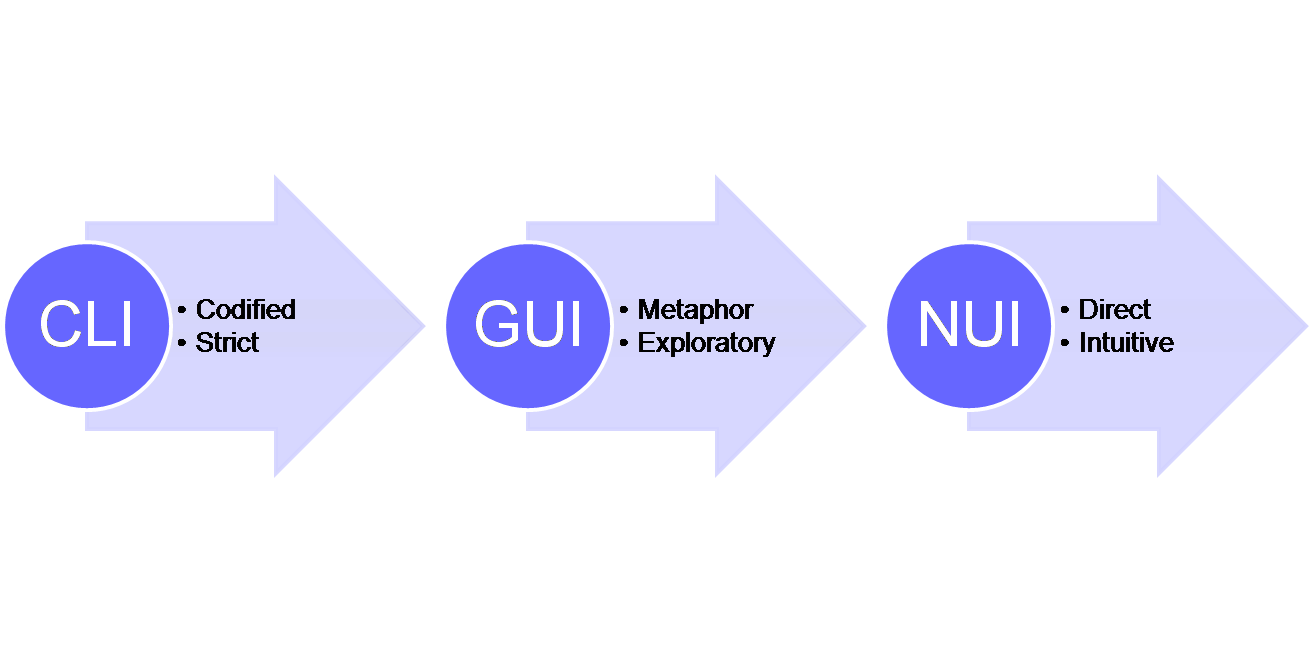
\includegraphics[width=0.9\textwidth]{images/nui.png}
\captionof{figure}{
Ewolucja interfejsów użytkownika
}
\small {źródło: https://en.wikipedia.org/wiki/Natural\_user\_interface }
\end{center}
\paragraph{}
Wiele nowych urządzeń próbuje implementować sterowanie interfejsem użytkownika za pomocą gestów (np. Microsoft Kinect\footnote{http://www.xbox.com/pl-PL/xbox-one/accessories/kinect-for-xbox-one}), czy też za pomocą myśli (np. Emotiv{\footnote{http://emotiv.com}). Na rynku widać duże zainteresowanie nową formą kontroli urządzeniami, zwłaszcza tymi bardziej naturalnymi dla człowieka. Jedankaże obecnie są to głównie eksperymenty nowej technologii. Nie ma na rynku obecnie wypracowanego popularnego standardu dostępu w grupie NUI.

\paragraph{}
W branży filmowej oraz gier wideo narasta trend używania nowych technologii do rozszerzania doznań jakie otrzymuje odbiorca.
W kinach odbywają są coraz częściej projekcje filmów stworzonych w technologii trójwymiarowej. Natomiast w ostatnim czasie pojawią się sale kinowe pozwalające na projekcję filmów trójwymiarowych wraz z dodatkowymi elementami takimi jak: drganie foteli, wiatr, dym, woda \footnote{http://cinema-city.pl/4dx-info}. Jednakże w obecnej chwili taki format rozrywki jest dość drogi, gdyż wymaga specjalnie przygotowanej sali kinowej oraz okularów, które pozwalają tworzyć iluzję przestrzenną. 

\subsection{Rozszerzona rzeczywistość}
\paragraph{}
Coraz bardziej popularne staje się pojęcie rozszerzonej rzeczywistości (ang. augmented reality). Jest to zbiór różnych technologii pozwalającej łączyć świat rzeczywisty z wirtualnym. Jest to jeszcze mało popularny sposób interakcji, lecz w ostatnim dziesięcioleciu rozwój (zarówno urządzeń jak i specjalistycznego oprogramowania) jest bardzo dynamiczny.
\paragraph{}
Pierwsze próby w tej dziedzinie odbywały się jeszcze w latach sześćdziesiątych amerykański naukowiec oraz artysta Myron Krueger prowadził badania nad wirtualną oraz rozszerzoną rzeczywistością. Jest on twórcą pojęcia środowiska responsywnego. ,,Jest to środowisko w którym działania użytkownika i odpowiada na nie w sposób przemyślany poprzez złożony system środków wizualnych i akustycznych, oraz dostosowuje się do powstałych w ten sposób nowych warunków środowiska.'' \footnote{http://www.techsty.art.pl/hipertekst/cyberprzestrzen/krueger.htm}. Stworzył on interaktywne instalacje takie jak Glowflow \footnote{http://dada.compart-bremen.de/item/artwork/1347}, Metaplay\footnote{http://dada.compart-bremen.de/item/artwork/1348} oraz Videoplace\footnote{http://dada.compart-bremen.de/item/artwork/1346}.

\begin{center}
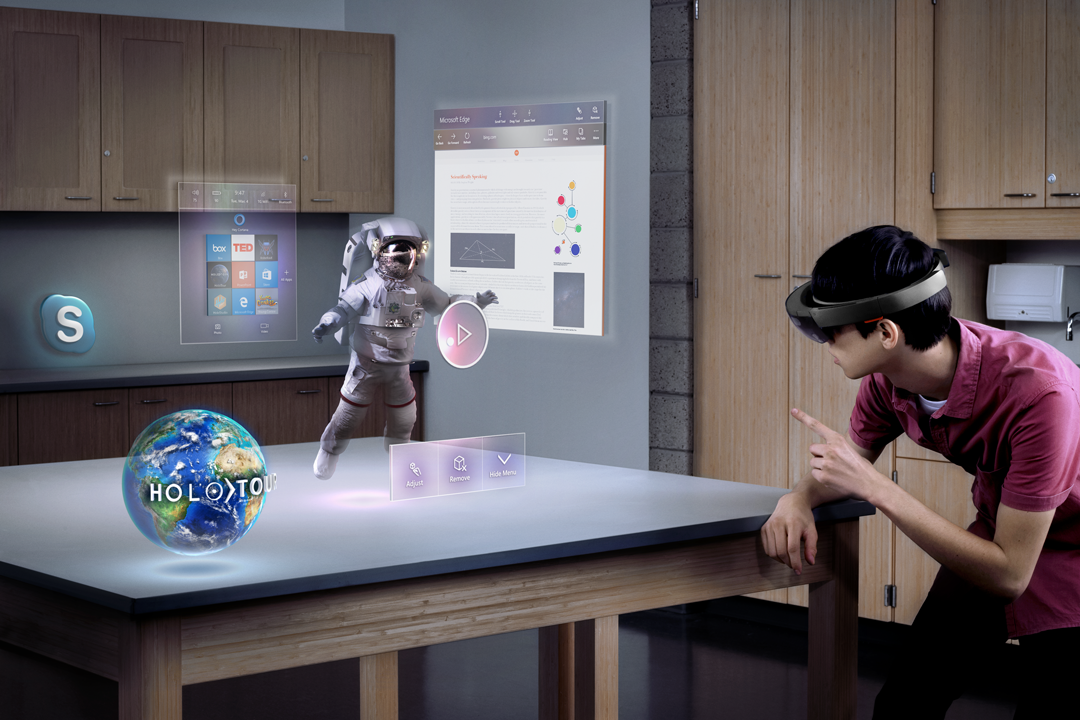
\includegraphics[width=0.9\textwidth]{images/hololens.png}
\captionof{figure}{
Wizualizacja Microsoft HoloLens
}
\small {źródło: https://www.microsoft.com/microsoft-hololens/en-us/why-hololens }
\end{center}
\section{Cel pracy}
\paragraph{}
Celem niniejszej pracy jest stworzenie platformy do budowania gier oraz interaktywnych animacji prezentowanej za pomocą rozszerzonej rzeczywistości sterowanej za pomocą zdalnego kontrolera. Praca zawiera przykłady różnych implementacji w technologiach z rodziny AR.

\paragraph{}
Przykłady zastosowanie zestawu aplikacji:

\begin{itemize}
	\item Prezentacje przestrzeni architektonicznych
	\item Rozrywka (np. gry)
	\item Reklama między innymi w miejscach użyteczności publicznych (np. centra handlowe)
\end{itemize}

\newpage
\section{Implementacje}
\paragraph{}
Rozdział prezentuje różne podejścia do stworzenia implementacji przykładowej sceny  w technologii rozszerzonej rzeczywistości.
Jako środowisko badawcze wybrano salę - labolatorium znajdującą się w Polsko-Japońskiej Akademii Technik Komputerowych. Salę tę wybrano, ponieważ znajduje się w podpiwniczeniu, co za tym idzie ilość światła dziennego jest znikoma. Pozwala to na bardzo łatwe stosowanie urządzeń projekcyjnych w ciągu dnia. Dodatkowo w sali znajduje się rura ciepłownicza poprowadzona po dwóch ścianach. Umiejscowienie tego elementu pozwala go wykorzystać do stworzenia wirtualnej sceny (np. animacja fal wody w środku rury).

\begin{center}
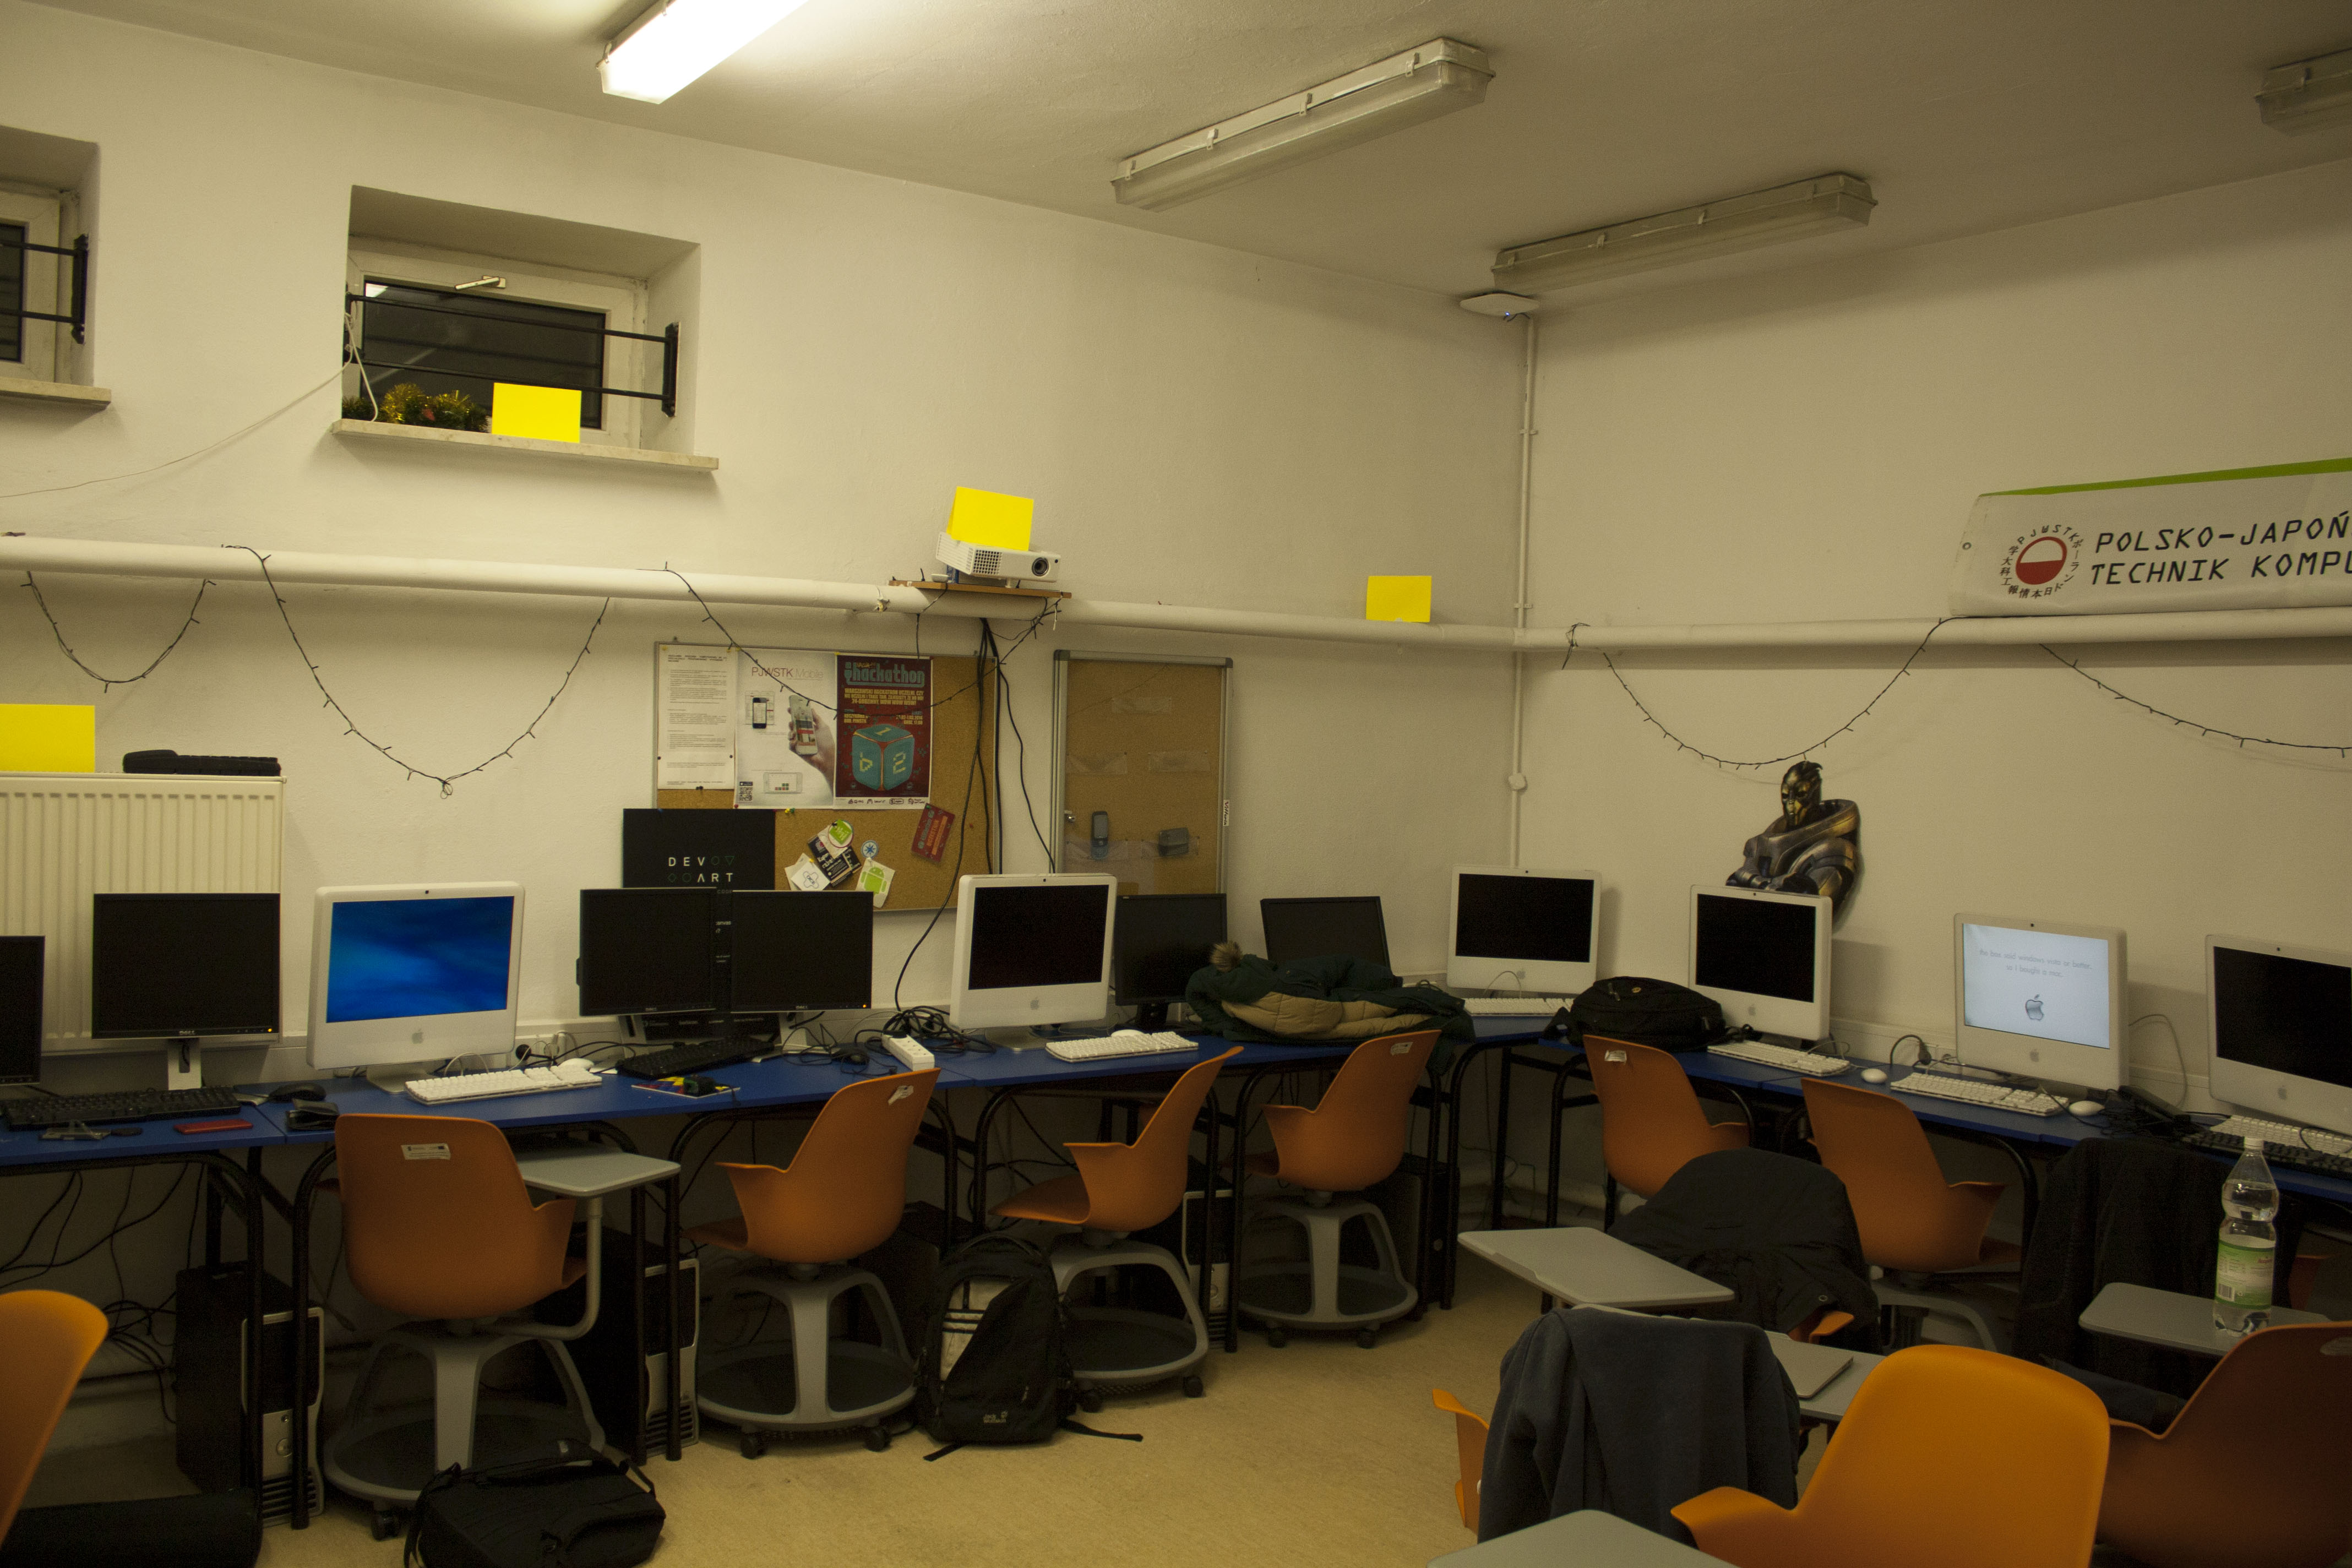
\includegraphics[width=0.9\textwidth]{images/s9.jpg}
\captionof{figure}{
Labolatorium PJATK
}
\end{center}

\paragraph{}
Głównym założeniem było stworzenie minigry opartej na grze z początku lat dziewięćdziesiątych o nazwie Lemmingi \cite{lemmings}. Pierwotnie gra została stworzona w 1991 roku na platformę Amiga.

Celem gry jest doprowadzenie grupy aktorów (tytułowych Lemmingów) do wyjścia (mety). Aktorzy automatycznie idą w jedną stronę. Każdemu z nich można włączyć jedną lub więcej umiejętność (np. umiejętność kopania, swobodnego spadania - spadochron). Aktorzy generowani są automatycznie w określonej sekwencji czasu.

\subsection{Implementacja w technologii hologramu}
\paragraph{}
Pierwotnym założeniem było stworzenie projektu za pomocą hologramu. Planowano wykorzystanie złudzenia optycznego stworzonego za pomocą światła na półprzezroczystej płaszczyźnie znajdującej się przed oczami odbiorcy. Analogiczną koncepcję prezentowało w przeszłości urządzenie Google Glass, a obecnie np. Microsoft Hololens lub Meta2.

Jednakże zamiast urządzenia nakładanego na głowę planowano użyć przezroczystą szybę znajdującą się na drzwiach wejściowych do labolatorium. Dzięki takiemu rozwiązaniu odbiór instalacji odbywałby się bez dodatkowych urządzeń, co za tym idzie interakcja byłaby bardziej naturalna.
Na szybie umieszczona zostałaby warstwa półprzezroczystej folii na której prezentowany byłby obraz za pomocą projektora multimedialnego ustawionego pod kątem około 30 stopni w górę w kierunku szyby. Projektor znajdowałby się na statywie w środku sali - technologia projekcja tylna.

Podczas eksperymentów próbowano wiele różnych folii oraz kilka ustawień projektorów. 

Zaobserwowano:
\begin{itemize}
	\item Umiejscowienie projektora pod kątem względem szyby powoduje bardziej naturalny obraz. Nie widać wtedy głównego strumienia światła z projektora (strumień światła nie jest prowadzony w linii prostej do odbiorcy), co za tym idzie  nie ma odczucia oślepienia.
    \item Użycie specjalnej folii do projekcji tylnej powoduje najlepszy odbiór. Inne folie przepuszczały zbyt małą ilość światła, bądź obraz z projektora był mało ostry.
    \item Użycie projektora w technologii LED okazało się lepsze, niż zastosowanie standardowego projektora multimedialnego. Mała odległość pomiędzy drzwiami, a urządzeniem pozwalała na użycie projektora z małą ilością lumenów.
\end{itemize}

\paragraph{}
Jednakże zrezygnowano z powyższego pomysłu, ponieważ napotkano problem nakładania obrazu z  elementami znajdującymi się w sali. Aby punkty wirtualne z ich rzeczywistymi odpowiednikami się nakładały i tworzyły spójny obraz (augumented reality) należałoby spoglądać przez szybę pod jednym wskazanym kątem. Co za tym idzie prawidłowy odbiór instalacji byłby zaburzony przez takie czynniki jak np. wzrost odbiorcy, kierunek wzroku czy też odległość od szyby. Urządzenia takie jak Microsoft Hololens niwelują ten problem poprzez stałe umiejscowienie półprzezroczystego ekranu w małej odległości od oka. 

\begin{center}
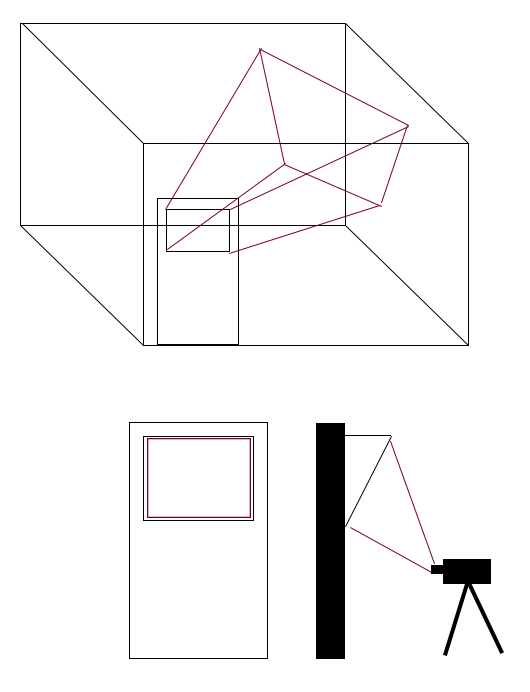
\includegraphics[width=0.9\textwidth]{images/hologramv1.png}
\captionof{figure}{
Poglądowy schemat działania hologramu
}
\end{center}

\begin{center}
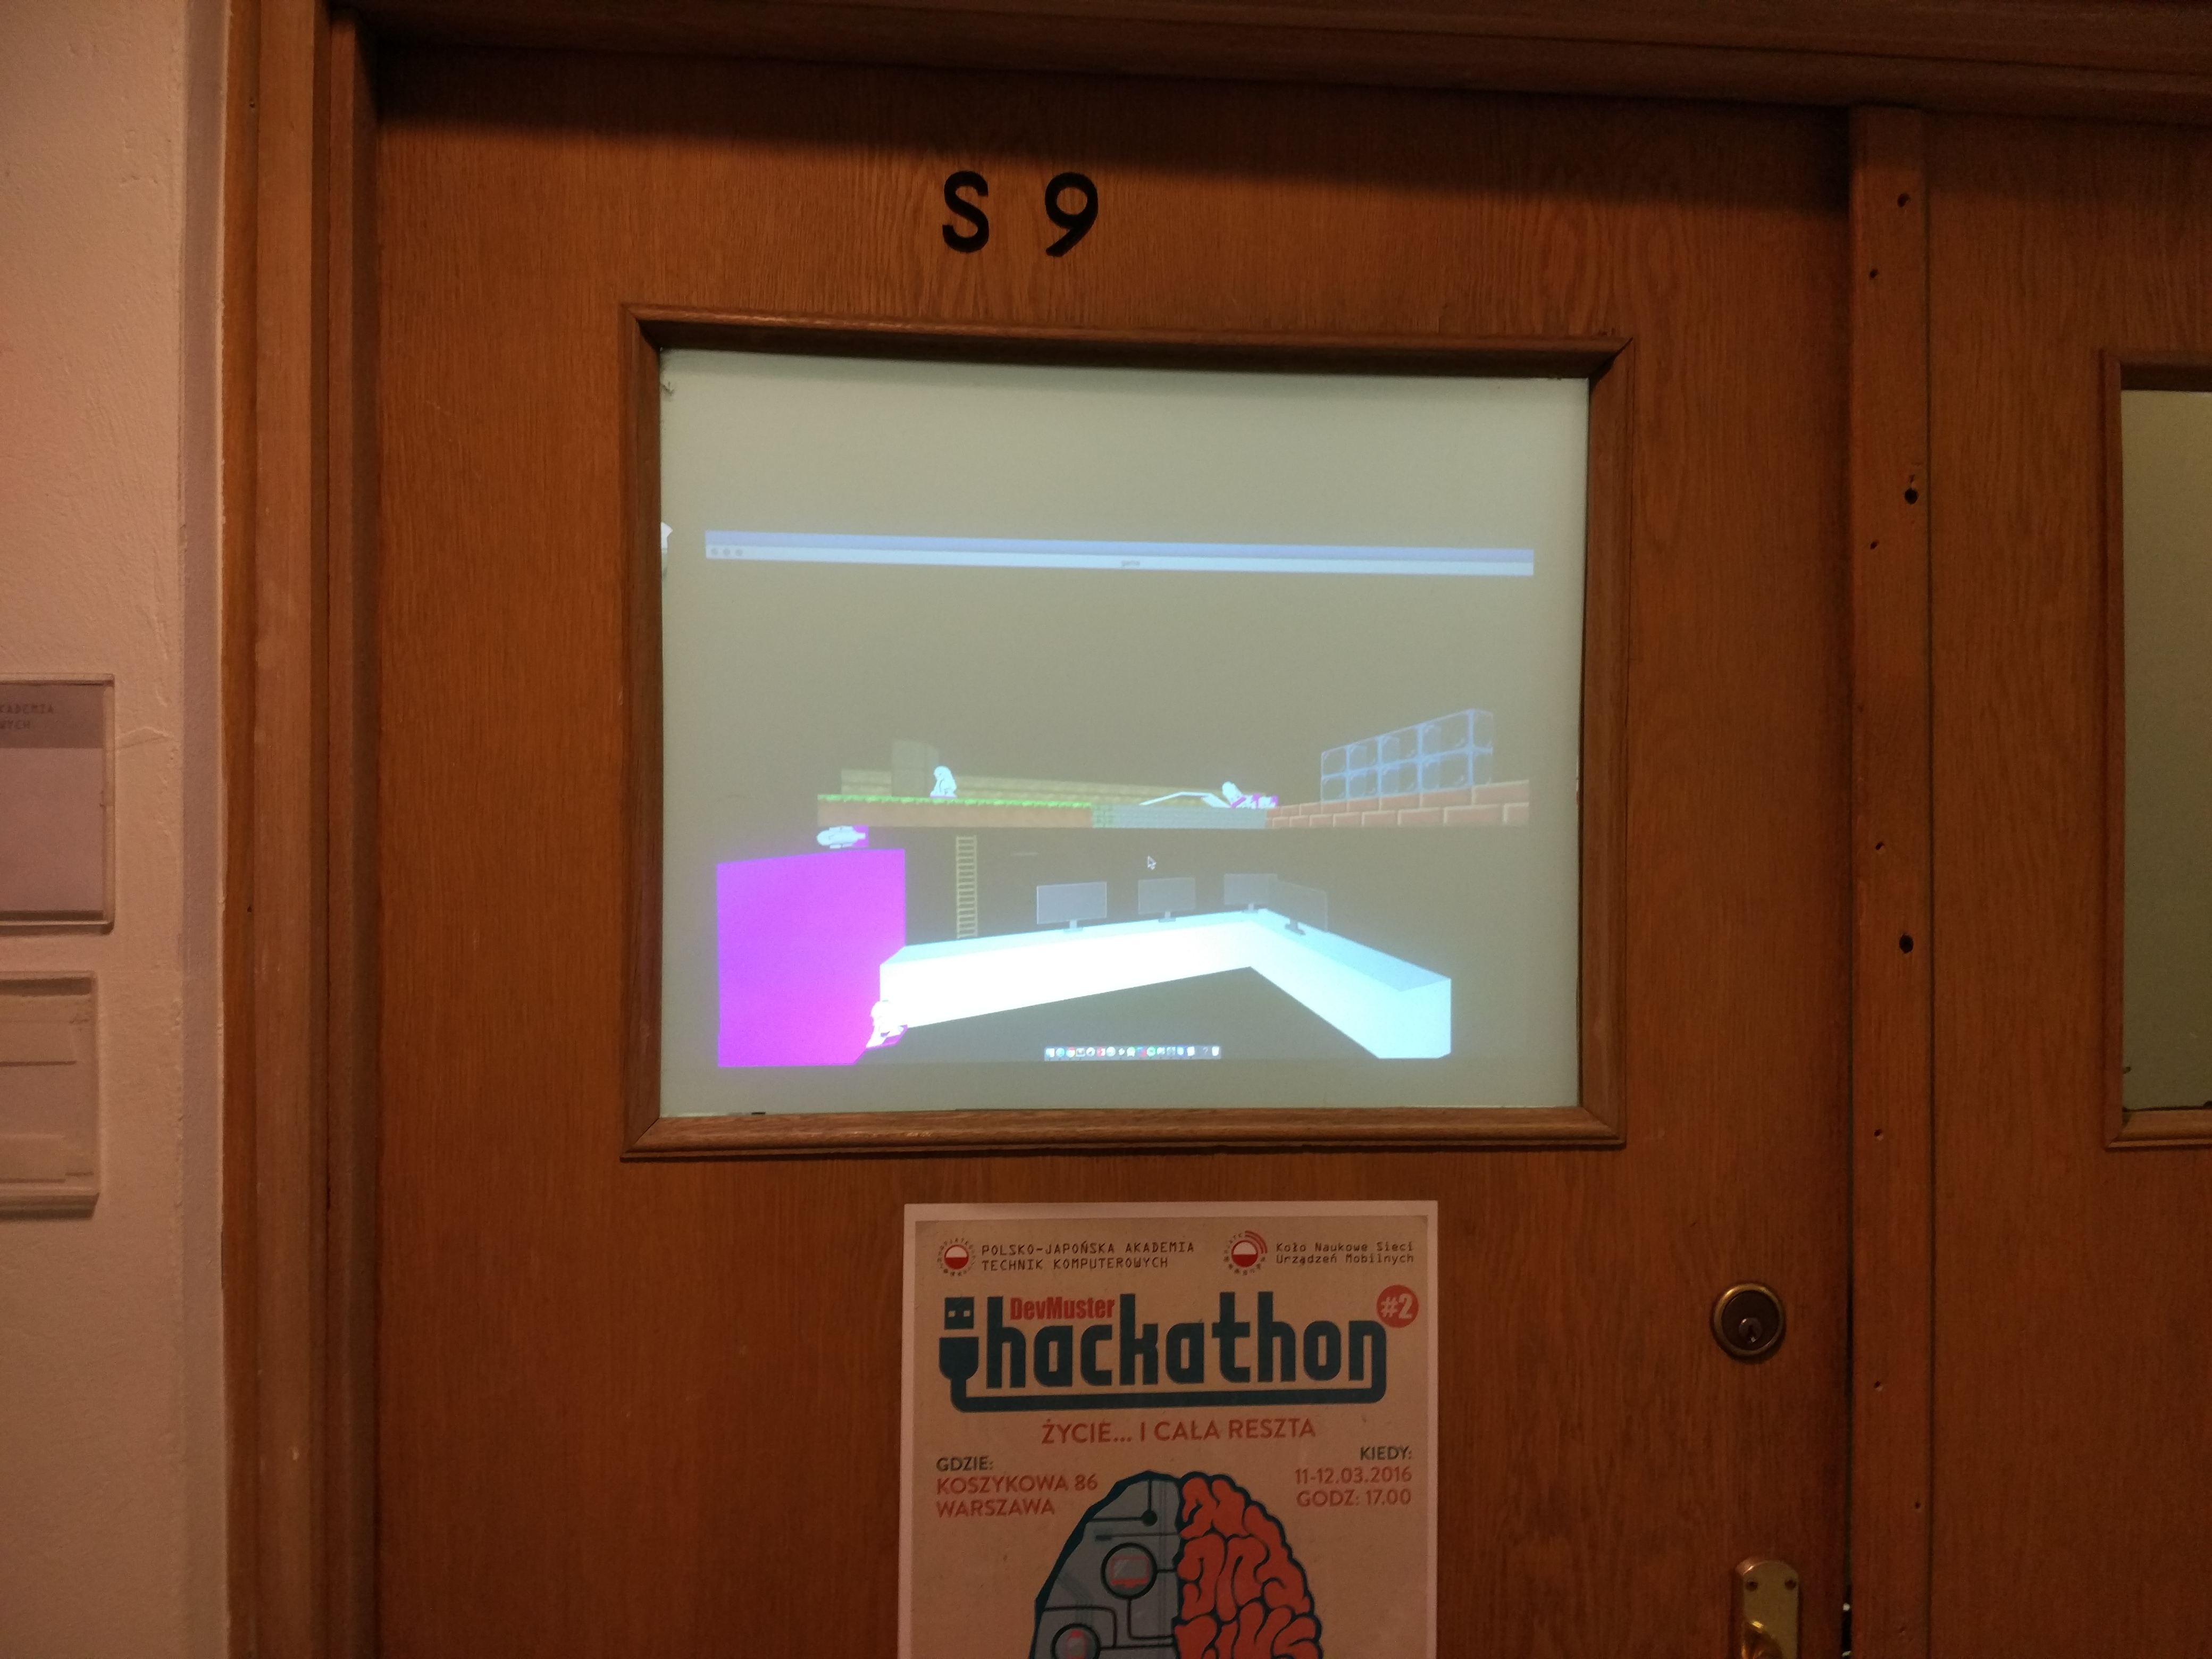
\includegraphics[width=0.9\textwidth]{images/drzwi.jpg}
\captionof{figure}{
Próba implementacji w laboratorium
}
\end{center}

\subsection{Implementacja w technologii mappingu 3d}
\paragraph{}
Kolejnym pomysłem było zastosowanie video mappingu 3d. Jest to technologia często spotykana w branży rozrywkowej (jako tło sceny koncertowej) oraz do prezentowania przestrzeni architektonicznych (zarówno wewnętrznych jak i zewewnętrznych), czy też pojazdów jak i innych mniejszych przedmiotów. 
\paragraph{}
Technologia polega na oświetlaniu rzeczywistego elementu  źródłem światła z projektora multimedialnego. Najlepsze efekty można uzyskać w zaciemnionych pomieszczeniach oraz przy lampach z dużą ilością lumenów. Dzięki temu za pomocą kolorów można pokazywać lub uniewidoczniać elementy przy wykorzystaniu koloru czarnego. Podczas projekcji ciemnego koloru ilość światła z projektora jest bardzo znikoma, co za tym idzie powstaje złudzenie, że element oświetlony światłem czarnym jest niewidoczny.
Przy realizacji większości instalacji takiego typu stosowany jest wcześniej przygotowany obraz wideo. Instalacje nie są interaktywne. Jednakże dzięki temu nawet zaawansowane animacje trójwymiarowe obciążają sprzęt komputerowy tylko podczas renderowania (zamiany obiektów trójwymiarowych na strumień video). Wprowadzenie elementów interaktywnych (np. sterowanie grą) mocno obcąża kartę graficzną komputera.
\paragraph{}
Założono, że projekcja odbywać będzie się na dwóch prostopadłych do siebie ścianach. Takie podejście wymaga dwóch projektorów. Jednakże obraz z nich musi być synchronizowany, ponieważ elementy interaktywne (np. postacie) będą przemieszczały się z jednej ściany na drugą. Zastosowanie dwóch komputerów wymagałoby stworzenia protokołu komunikacyjnego. Założono, iż zastosowany będzie jeden komputer z wydajną kartą graficzną, która obsłuży dwa źródła wyjścia.

\begin{center}
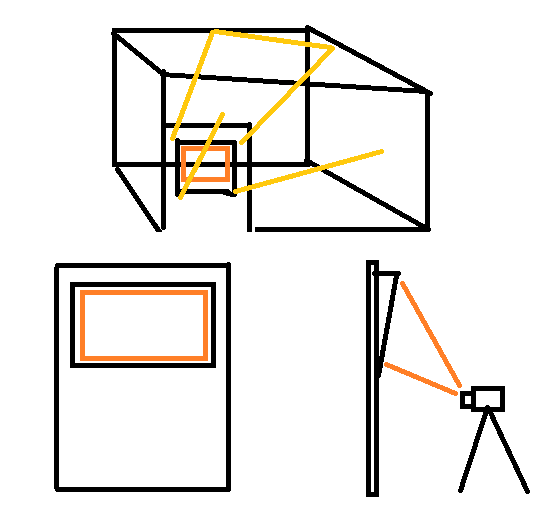
\includegraphics[width=0.9\textwidth]{images/mappingv1.png}
\captionof{figure}{
Poglądowy schemat działania - mapping
}
\end{center}

\begin{center}
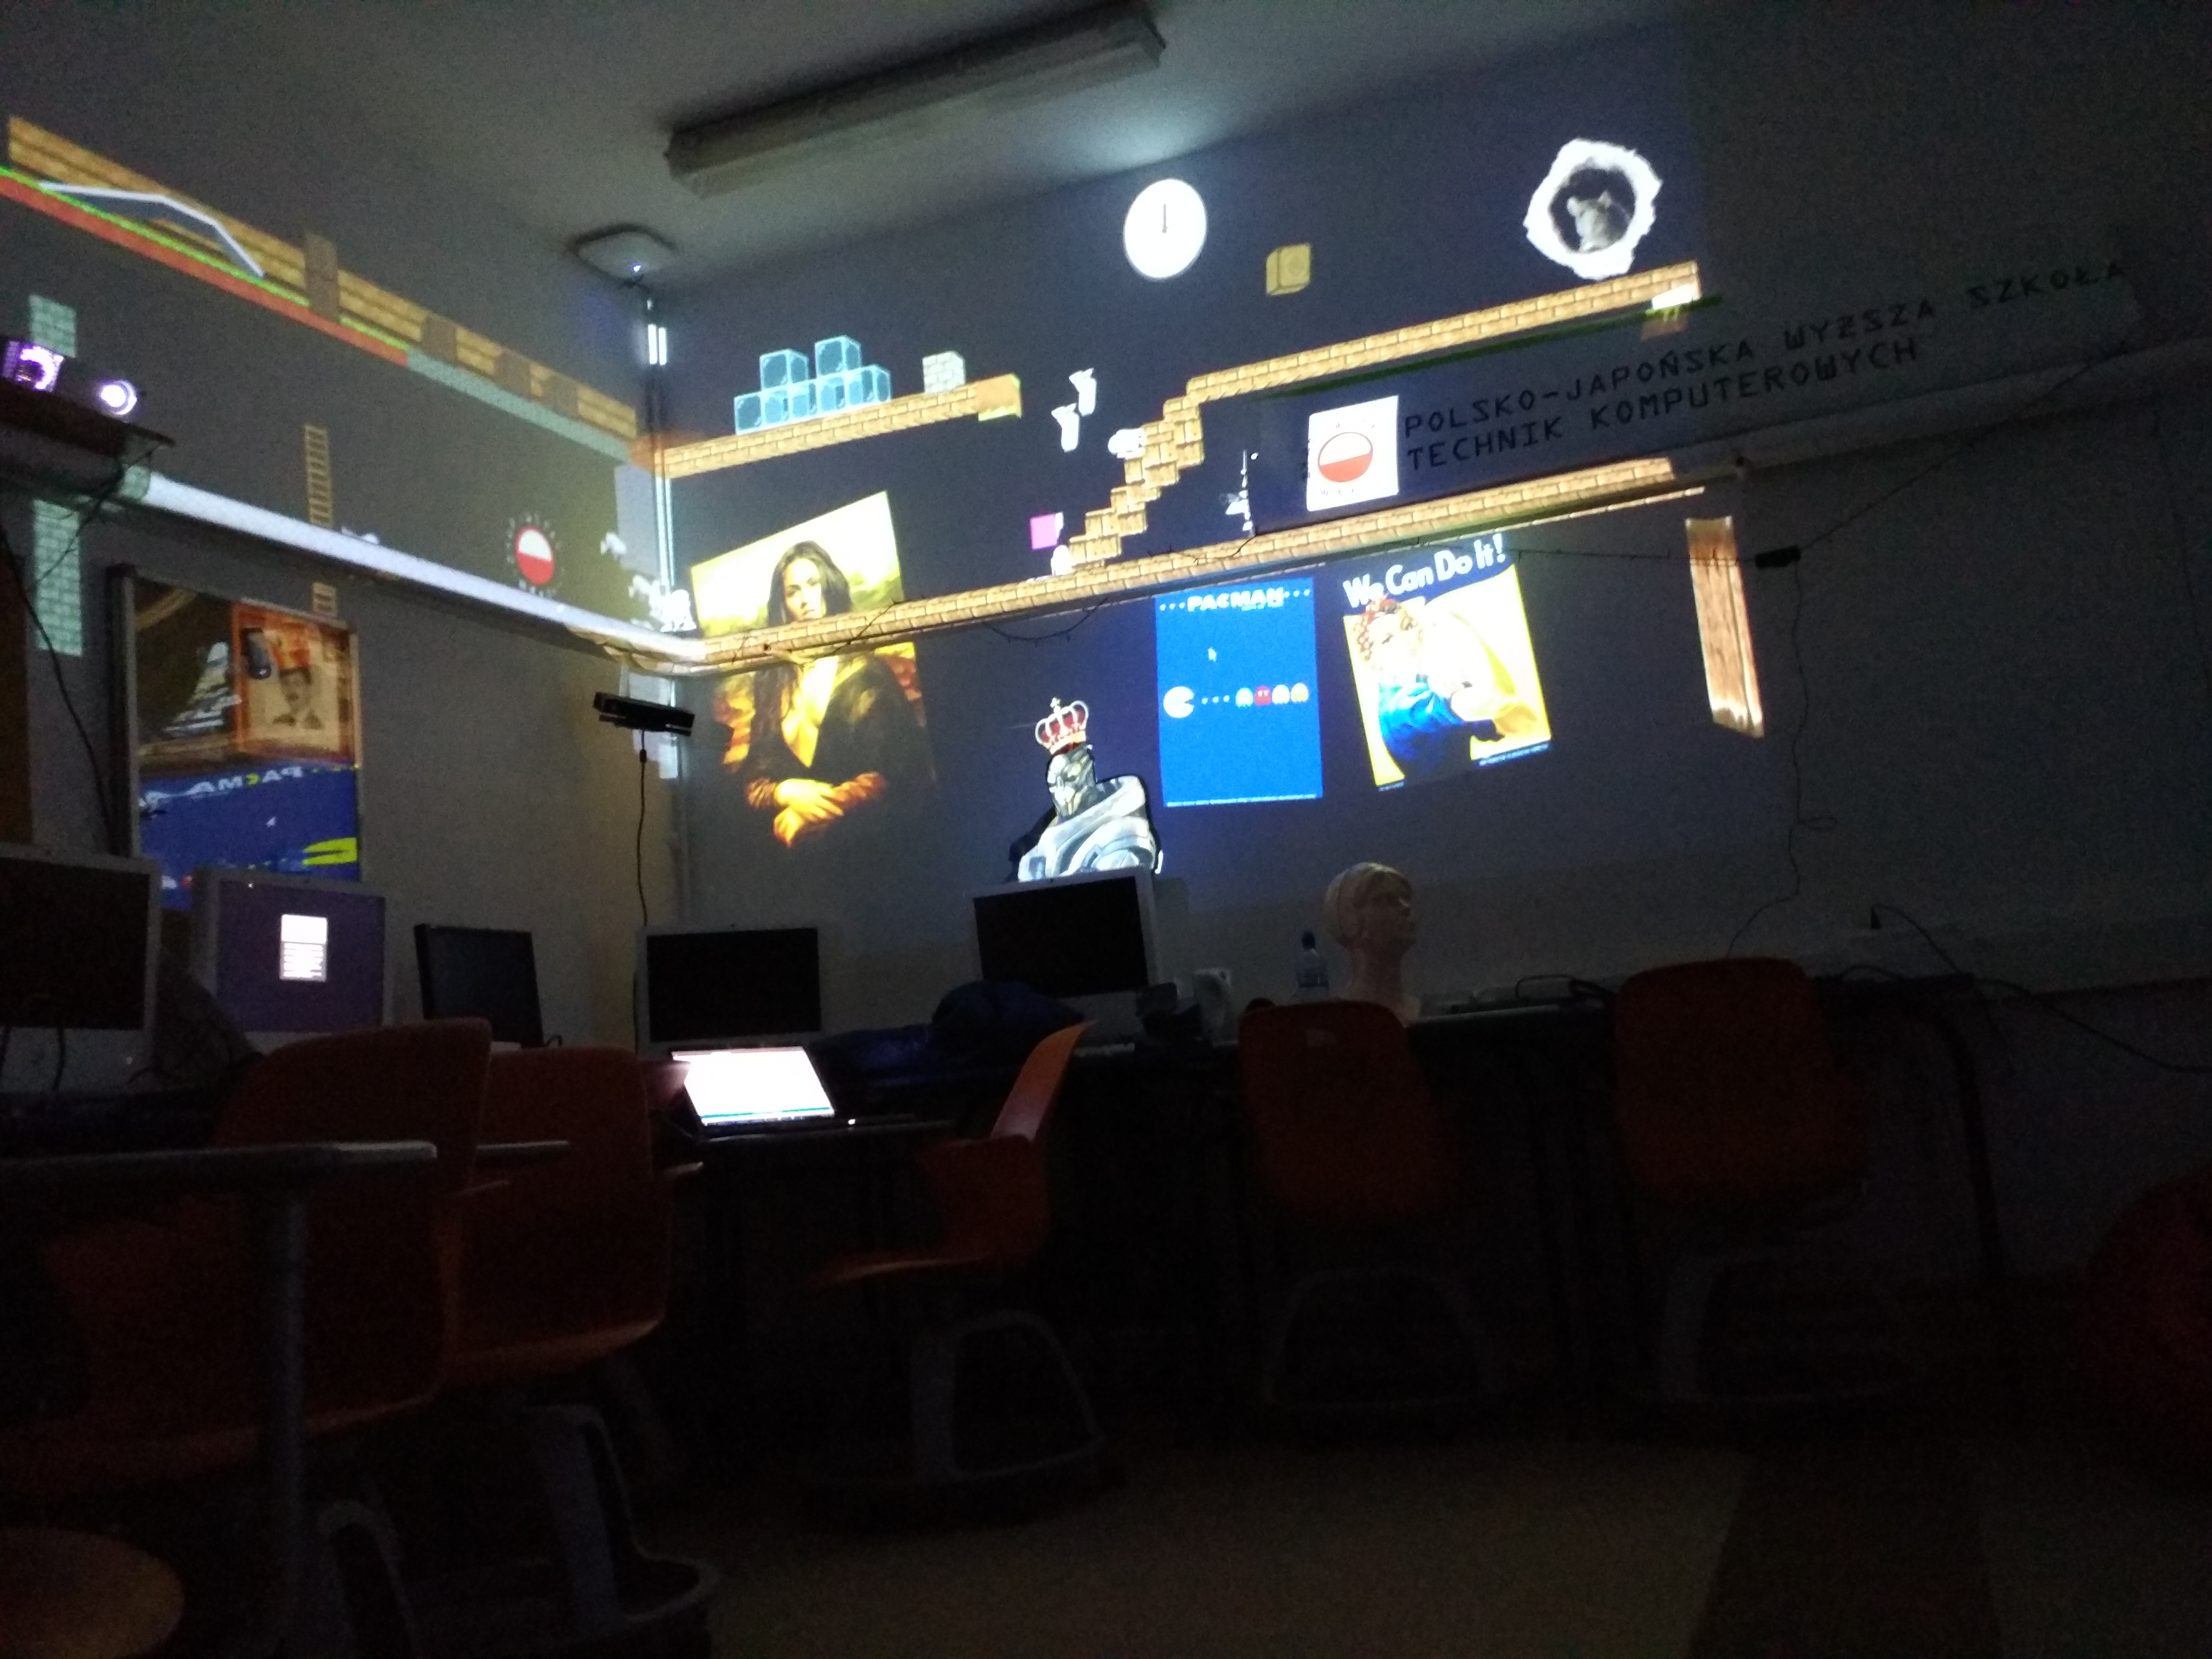
\includegraphics[width=0.9\textwidth]{images/implementacja.jpg}
\captionof{figure}{
Implementacja w laboratorium
}
\end{center}

\paragraph{}
Zaobserowano:
\begin{itemize}
	\item Efekty wizualne są odpowiednie, jednakże zauważalny jest brak głębi obrazu. Wszystkie elementy są dwuwymiarowe.
	\item Bardzo ważnym aspektem jest jakoś lampy projektora i jego umiejscowienie. Nawet drobne przesunięcie projektora w stosunku do ściany może zaburzyć odbiór instalacji.
\end{itemize}

\newpage
\section{Wykorzystane technologie}

\subsection{Unity}
\paragraph{}
Unity jest obecnie najpopularniejszą platformą do tworzenia gier (zarówno trójwymiarowych jak i dwuwymiarowych) na wiele platform sprzętowych. Silnik ten korzysta z API Direct3D (na urządzeniach Windows) oraz OpenGL.
\subsubsection{Dlaczego Unity}
\paragraph{}
Najnowsza wersja posiada natywne wsparcie do rozszerzonej oraz wirtualnej rzeczywistości. Dodatkowo większość projektów budowanych w oparciu o ideologoię AR dostarcza Software Development Kit właśnie dla Unit, co za tym idzie możliwe jest łatwe porównanie różnych implementacji.
Narzędzie te posiada prosty, ergonomiczny interfejs co ułatwia pracę.
\paragraph{}
Bardzo pomocnym dodatkiem do narzędzia jest ,,Assets Store''. Jest to wirtualny sklep z komponentami do tworzenia gry. W projekcie zastosowałem tekstury i obiekty 3D pochodzące z tego źródła.

Dodatkowo silnik ten wspiera import modeli trójwymiarowych w bardzo dużej ilości specjalistycznych rozszerzeń plików.

\subsubsection{Alternatywne rozwiązania}
 \begin{tabular}{|c|c|c|}
 \hline
 \ & Unity & Unreal Engine \\ 
  \hline
 Wsparcie języków programowania & C\#, JavaScript, Boo & c++ \\  
  \hline
 Obsługa wielu ekranów & Tak & Nie \\
 \hline  
  Wsparcie dla Google Cardboard & Tak & Nie \\
  \hline   
  Popularność/społeczność & duża &  znikoma \\
  \hline   
\end{tabular}
\captionof{table}{Porównanie silników gier}

\subsubsection{Wybór języka programowania}
\paragraph{}
Środowisko Unity wspiera obsługę skryptów (animacje oraz logika biznesowa) w kilku językach programowania: C\#, UnityScript (zmodyfikowana wersja JavaScript)  oraz w przeszłości Boo. Podjęto decyzję, by w projekcie użyć język C\#, gdyż ów język jest najbardziej stabilny, posiada najbardziej rozbudowaną dokumentację oraz jest to najpopularniejszy język w specjalistycznej literaturze. Dodatkowym udogodnieniem  jest to, iż  język posiada wiele wbudowanych klas (np. do obsługi połączeń TCP) oraz niezliczoną ilość zewnętrznych bibliotek.
\subsubsection{Unity IDE}
\paragraph{}
Środowisko Unity jest multiplatformowe. Aplikacje można używać na dowolnym sytemie operacyjnym. Jednakże edycja skryptów odbywa się za pomocą zewnętrznego narzędzia. W systemie Mac OS X jest to MonoDevelop, natomiast w systemie Windows jest to VisualStudio w wersji Community. Opisywana aplikacja początkowo była tworzona na systemie Mac OS X, jednakże kołopoty ze środowiskiem MonoDevelop spowodowały decyzje o przeniesieniu środowiska na system Windows. Subiektywnie mogę stwierdzić, że stabilność oraz komfort pracy jest dużo lepszy w systemie Windows.
Dodatkową alternatywą dla MonoDevelop może okazać się Visual Studio Code. Jest to prosty multiplatformowy edytor posiadający obsługę języka C\# .

\subsubsection{Licencja i koszty}
\paragraph{}
Unity jest zamkniętym, licencjonowanym oprogramowaniem. Darmowa wersja (Personal Editon) pozwala na nielimitowane użycie, jednakże jest to okrojona edycja. Szersze informacje o ograniczeniach wersji Personal zawarte są w kolejnych rozdziałach. Licencja pozwala na komercyjne użycie przy limicie zarobków na poziomie stu tysięcy dolarów.
Komercyjna wersja (Professional Edition) jest płatna w modelu subskrypcyjnym (75 dolarów za miesiąc)\footnote{https://store.unity3d.com/subscribe}.
Na potrzeby opisywanego projektu zastosowano Unity w wersji Personal Edition.

\subsection{Android}
\paragraph{}
Naturalnym wyborem technologii przy tworzeniu aplikacji na urządzenie sterujące byłoby Unity, gdyż te środowisko pozwala na kompilacje kodu na urządzenia mobilne(systemy: iOS, Android, Windows Phone, Tizen itp\footnote{https://unity3d.com/unity/multiplatform}). Jednakże Unity w wersji Personal Edition nie pozwala na uruchomienie warstwy sieciowej na urządzeniach mobilnych.
\paragraph{}
Na potrzeby implementacji przykładowego urządzenia sterującego wybrano platformę Android, gdyż ma ona największy udział w rynku.\footnote{https://www.netmarketshare.com/operating-system-market-share.aspx?qprid=10\&qpcustomd=1} Proces tworzenia aplikacji na tą platformę przebiega w języku Java.

\subsection{Komunikacja sieciowa}
\paragraph{}
Największym wyzwaniem było stworzenie dwukierunkowego protokołu komunikacyjnego pomiędzy serwerem (aplikacja napisana w środowisku Unity) oraz dowolnym kontrolerem lub w przyszłości innym urządzeniem wysyłającym dane do aplikacji. Podstawowym założeniem było to iż, kontrolerem gry może być standardowy telefon komórkowy. Dodatkowo w przyszłości planowana jest rozbudowa o zdalne sterowanie za pomocą przeglądarki internetowej. Pierwotnie rozważane było użycie Bluetooth, jednak ograniczyłoby to zdalne sterowanie. Podjęto decyzję projektową o użyciu połączenia sieciowego. Rozważano następujące protokoły:

\subsubsection{UNET}
\paragraph{}
Unity wspiera natywną obsługę multiplayer - UNET, jednakże jest to zamknięty protokół. Komunikacja możliwa jest tylko pomiędzy aplikacjami stworzonymi w tym środowisku.

\subsubsection{HTTP (SOAP, REST)}
\paragraph{}
Komunikacja za pomocą HTTP (protokoły komunikacyjne takie jak np. SOAP, REST) są bardzo często spotykane. Jest to standard aplikacji internetowych. HTTP nadaje się do przesyłu dużych wolumenów danych, jednak niezbyt dobrze sprawdza się przy małych, lecz częstych połączeniach pomiędzy klientem, a serwerem. Duży narzut czasowy może spowodować transformacje danych do oraz z formatu JSON lub XML. Jednakże dużą zaletą wspomnianych protokołów jest prostota implementacji w większości języków programowania, gdyż są już gotowe komponenty.
\subsubsection{WebSocket}
\paragraph{}
Zdecydowano, że najlepszym rozwiązaniem będzie użycie protokołu komunikacyjnego TCP, a dokładniej technologii WebSocket, która pozwala na dwustronną komunikację na zasadzie klient-serwer. Jest to protokół połączeniowy.
W celu ułatwienia implementacji wybrano bibliotekę socket.io\footnote{http://socket.io/}. Główną jej zaletą jest możliwość nasłuchiwania i emitowania danych do wszystkich odbiorców z poszczególnej grupy. Pozwala to na stworzenie platformy, która będzie mogła w przyszłości obsługiwać wiele instancji gry lub kilka kontrolerów jednocześnie. Dodatkowym udogodnieniem jest to, iż popularność tej biblioteki sprawiła, że posiada ona wiele implementacji w różnych językach programowania.
Jako Middleware - pośrednik pomiędzy grą, a kontrolerem wybrano technologię Node.js. Zbudowano lekki szkielet, obsługujący połączenia wielokierunkowe. Dzięki wydzieleniu Middleware żadna z instancji gry lub kontrolera nie pełni roli serwera co powoduje wzrost wydajności danej platformy. Dodatkowo w przyszłości można rozbudować serwer o możliwość przechowywania zapisanego stanu gry lub np. ilości punktów zebranych przez użytkownika.
\newpage
\section{Aplikacja główna}
\paragraph{}
Głównym założeniem aplikacji w Unity jest stworzenie wirtualnego świata składającego się z wizualizacji dwóch ścian oraz elementów znajdujących się na nich. Po wyznaczonych elementach poruszać się będą aktorzy, czyli postacie gry.

\subsection{Świat gry}
\paragraph{}
Na wizualizacji dwóch ścian znajdują się przeszkody, czyli wirtualne platformy zbudowane z prostopadłościanów. Część z nich nakłada się na rzeczywiste elementy - na przykład rura ciepłownicza. Na platformach się elementy aktywne, które reaguję na interakcje z aktorem. Aby pokonać przeszkodę, będzie musiał on wykonać jedną z dostępnych w danej chwili akcji (np. rozbicie szklanego elementu czy też wykopanie).

\begin{center}
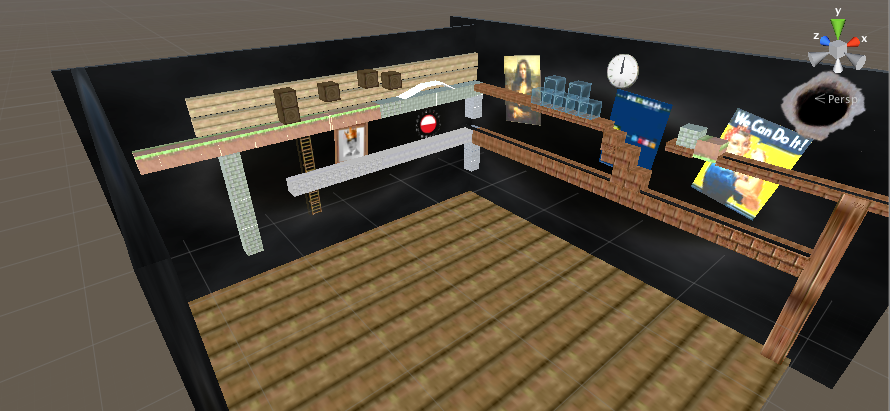
\includegraphics[width=1\textwidth]{images/swiatgry.png}
\captionof{figure}{
Model w środowisku Unity
}
\end{center}

\subsection{Aktorzy}
\paragraph{}
Aktor to element interaktywny w grze. Podczas jej inicjalizacji aktor (prefabrykat z gotowym trójwymiarowym modelem) zaczyna się poruszać w jednym kierunku. Zadaniem gracza (za pomocą kontrolera) jest nadanie jednej z wielu umiejętności, tak aby aktor mógł przejść z miejsca startu do końca planszy.

Zaimplementowane możliwości aktora to:

\begin{itemize}
  \item wykopanie elementu
  \item spadochron - swobodne spadanie
  \item rozbicie za pomocą kilofa elementu
  \item umiejętność skakania
  \item umiejętność zatrzymania się i ponownego swobodnego przechodzenia
  \item reset - powrót do pozycji startowej
\end{itemize}

\begin{lstlisting}[language=CSharp]
public static Vector3 lemmingPosition = new Vector3 (1205.9F, 103.4F, -4996.9F);
private static Vector3 jumpSize = new Vector3 (0, 200F, 0F);
\end{lstlisting}
\captionof{lstlisting}{
  Konfiguracja pozycji początkowej i siły skoku
}

\begin{lstlisting}[language=CSharp]
public void SendInfo() {
  Network.SendMessage("hasax_"+this.hasAx);
  Network.SendMessage("hassh_"+this.hasSh);
  Network.SendMessage("hasdrabina_"+this.drabina);
  Network.SendMessage("isMove_"+this.isMove);
}
\end{lstlisting}
\captionof{lstlisting}{
  Przykład wysyłania komunikatów do serwera
}

\paragraph{}
Podczas tworzenia nowej instancji klasy Aktora zapisywana ona jest do listy statycznej wszystkich dostępnych na daną chwilę obiektów (podczas usunięcia z planszy element również znika z listy). Ma to na celu możliwość implementacji w kontrolerze możliwości wyboru aktywnego aktora.

\begin{lstlisting}[language=CSharp]
public static void GetNext() {
Debug.Log ("get next");
if (Lemming2.activeEl == null) {
  Lemming2.activeEl = Lemming2.lista [0];
} else {
  int i = Lemming2.lista.IndexOf(Lemming2.activeEl);
  if (i < Lemming2.lista.Count - 1) {
    Lemming2.activeEl = Lemming2.lista [i + 1];
  } else {
    Lemming2.activeEl = Lemming2.lista [0];
  }
}

Lemming2.activeEl.SendInfo ();
}
\end{lstlisting}
\captionof{lstlisting}{
  Wybór aktywnego aktora.
}

\paragraph{}
Każdy z aktorów posiada detekcję kolizji z innymi elementami za pomocą nadpisania wbudowanych metod w środowisko Unity. Są to: OnTriggerEnter, OnTriggerExit, OnCollisionEnter, OnCollisionExit. Kolizja od triggera, różni się tym, iż metody OnCollsion współpracują tylko z elementami, które posiadają zaimplementowaną fizykę (np. spadający element platformy), natomiast trigger to można być dowolny element, nie posiadający ,,ciała'' (np. ściana).
\newline
W celu uproszczenia detekcji kolizji z innymi elementami wprowadzono czarne prostopadłościany emitujące rzeczywiste ściany. Są one koloru czarnego, dzięki temu projektor emitujący obraz w tych miejscach nie wyśle światła widzialnego. Natomiast dzięki takiemu zabiegowi możliwe jest zamodelowanie w środowisku unity kolizji z rzeczywistymi elementami.

\begin{center}
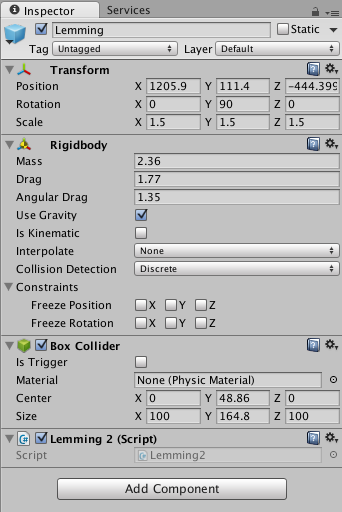
\includegraphics[width=0.7\textwidth]{images/aktor.png}
\captionof{figure}{
Konfiguracja aktora
}
\end{center}

\subsection{Prefabrykaty}
\paragraph{}
W Unity możliwe jest używanie prefabrykatów (Prefabs\cite{prefab}). Są obiekty lub grupy obiektów, które służą do wielokrotnego wykorzystywania. W Projekcie założono, że wszystkie reużwalne komponenty (dziedziczone pomiędzy scenami) będą prefabrykatami.
Dodatkowo aktorzy gry (generowane dynamicznie) są również prefabrykatami. Instancje aktora są tworzone podczas działania aplikacji.
\newline
\subsection{Kamery}
\paragraph{}
Ważnym elementem gry są wirtualne kamery. To z nich renderowane jest ujęcie, czyli obraz gry. W projekcie zastosowano dwie kamery. Podczas konfiguracji uruchomieniowej należy ustawić by każda z kamer była wyświetlana na oddzielnym źródle obrazu (monitor, projektor). Dzięki temu projekt można uruchomić na dwóch prostopadłych ścianach.
Jako tło sceny wybrano jednolity kolor czarny, ponieważ ten kolor nie jest prezentowany podczas projekcji. Światło z projektora jest w tym miejscu znikome, wręcz niewidoczne. Stosując taki prosty zabieg można łączyć elementy rzeczywiste (np. rura czy inne elementy stałe znajdujące się w laboratorium) z wirtualną rzeczywistością.

\begin{center}
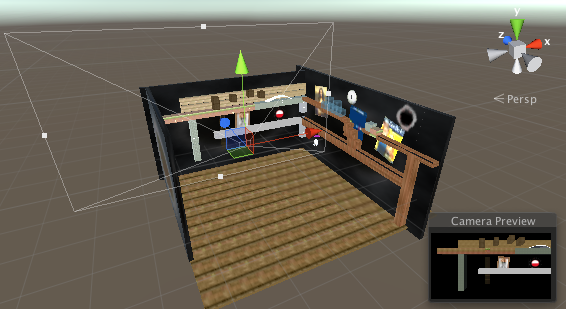
\includegraphics[width=1\textwidth]{images/kamera1.png}
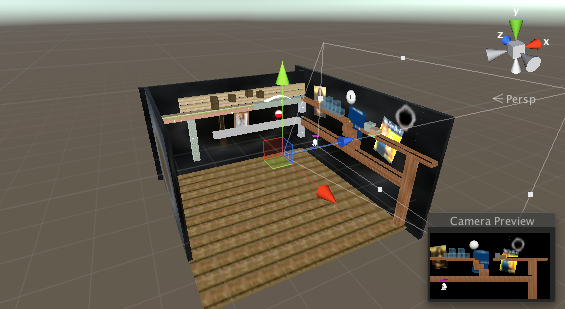
\includegraphics[width=1\textwidth]{images/kamera2.png}
\captionof{figure}{
Ujęcie wirtualnych kamer
}
\end{center}

\paragraph{}
Środowisko Unity domyślnie nie ma włączonej opcji wspierania wielu kamer jednocześnie. Do opisywanego prefakbrykatu należy dodać abstrakcyjny GameObject z poniższym prostym skryptem, który przy uruchomieniu skompilowanej gry sprawdza dostępność sprzętową ekranów.
\newline
\newline
\begin{lstlisting}[language=CSharp]
using UnityEngine;
using System.Collections;

public class DisplayScript : MonoBehaviour
{
  void Start()
  {
    Debug.Log("displays connected: " + Display.displays.Length);
    if (Display.displays.Length > 1)
      Display.displays[1].Activate();
    if (Display.displays.Length > 2)
      Display.displays[2].Activate();
  }
}
\end{lstlisting}
\captionof{lstlisting}{
  Prosta aktywacja ekranów
}

\paragraph{}
Podczas testów uruchomieniowych przy dwóch kamerach występował problem z wydajnością karty graficznej. Zwłaszcza gdy do komputera podłączano dwa zewnętrzne ekrany po złączach cyfrowych (np. HDMI, DisplayPort, DVI). Finalnie problem rozwiązano wydajniejszym komputerem, jednakże pośrednim rozwiązaniem było użycie portu VGA, który jest mniej obciążający dla karty graficznej.

\subsection{Światło}
\paragraph{}
Kolejny prefabrykat stworzono by zachować spójność w oświetleniu trójwymiarowej sceny. Służy on do zgrupowania wszystkich źródeł wirtualnego światła. Jest to element bez zawartej logiki biznesowej. Stworzono go w celu zachowania porządku w projekcie.


\subsection{SocketIO}
\paragraph{}
Jest to prefabrykat dostarczony jako komponent implementacji Socket.io w bibliotece Asset Store. Jest on udostępniony na licencji Open Source.  Musi być on umiejscowiony w każdej scenie, która korzysta z połączenia sieciowego. Umiejscowienie jest dowolne, gdyż jest to prefabrykat abstrakcyjny (nie posiada graficznej reprezentacji w trójwymiarowym modelu). W prefabrykacie wywołano skrpyt \texttt{SocketIOComponent}, który odpowiada za inicjalizacje komunikacji sieciowej.

\subsection{Network}
\paragraph{}
Jest to kolejny prefabrykat abstrakcyjny, który służy do uruchomienia klasy \texttt{Network}odpowiadającej za implementacje metod służących do dwustronnej komunikacji.
Prefabrykat ten jest nierozerwalnie złączony z SocketIO, gdyż bezpośrednio korzysta z metod dostarczonych przez tą bibliotekę.


\begin{lstlisting}[language=CSharp]
private SocketIOComponent socket;

// Use this for initialization
void Start () {
  GameObject go = GameObject.Find("SocketIO");
  socket = go.GetComponent<SocketIOComponent>();

  socket.On("open", InitGame);
  socket.On("button", Button);
}
\end{lstlisting}
\captionof{lstlisting}{
  Inicjalizacja skryptu
}

\paragraph{}
Na początku wyszukiwany jest obiekt gry o określonej nazwie, a następnie pobierany komponent, czyli obiekt klasy. Warto pamiętać, ze połączenie inicjalizowane jest już przy uruchomieniu, więc nie ma potrzeby ,,ręcznego'' zestawiania warstwy sieciowej.
\newline
Metoda On w klase \texttt{SocketIOComponent} odpowiada za nasłuchiwanie serwera. Jako pierwszy parametr przyjmuje ciąg znaków określający nazwę metody. Natomiast drugi to referencja do metody, która wywoła się podczas wywołania akcji o nazwie wynikającej z pierwszego parametru.
\newline
Na potrzeby łatwiejszego zarządzania zdarzeniami i uniknięcia błędów w nazwach przycisków stworzono enum, zawierający nazwy obsługiwanych przycisków. Wszystkie metody odpowiadające za komunikację, a zwłaszcza za zarządzanie stanami oraz nazwami przycisków powinny przyjmować w parametrze opisywany atrybut wyliczalny.
\newpage

\begin{lstlisting}[language=CSharp]
using System;

namespace AssemblyCSharp
{
  public enum ButtonEnum
  {
    BUTTON1, BUTTON2, BUTTON3, BUTTON4, BUTTON5, BUTTON6, BUTTON7, BUTTON8, BUTTON9, BUTTON10
  }
}

\end{lstlisting}
\captionof{lstlisting}{
  Definicja przycisków.
}

\paragraph{}
Metoda zarejestrowana pod nazwą \texttt{open} wywoła się przy udanym zestawieniu połączenia. Jest to najlepsze miejsce do wstępnej konfiguracji planszy gry oraz przycisków w kontrolerze.

\begin{lstlisting}[language=CSharp]
public void InitGame(SocketIOEvent e)
{
  socket.Emit("register_game");
  EnableButton(ButtonEnum.BUTTON1);
  SetText(ButtonEnum.BUTTON1, "Nazwa 1");
  DisableButton(ButtonEnum.BUTTON2);
}
\end{lstlisting}
\captionof{lstlisting}{
  Inicjalizacja komponentów
}

\paragraph{}
Powyższy przykład inicjalizacji pokazuje emitowanie akcji do serwera o nazwie \texttt{register\_game}. Służy on do zarejestrowania gry na serwerze. Od tego czasu wszystkie akcje z kontrolera (np. wciśnięcie przycisku) będzie emitowane do gry.
Dodatkowo ukazano wstępną konfigurację przycisków: Uaktywnienie przycisku pierwszego, ustawienie określonej nazwy oraz wyłączenie przycisku drugiego.

\subsection{Budowanie zapytania}

\begin{lstlisting}[language=CSharp]
public void SetText(ButtonEnum btn, string text) {
  Dictionary<string, string> dic = new Dictionary<string, string> ();
  dic.Add ("name", btn.ToString());
  dic.Add ("text", text);
  socket.Emit ("set_text", new JSONObject (dic));
}
\end{lstlisting}
\captionof{lstlisting}{
  Przykładowe zapytanie do gra - kontroler
}

\subsection{Replikator}
\paragraph{}
Replikator to komonent do tworzenia nowych instancji aktora. Ma na celu cykliczne dodawanie kolejnych obiektów aktora w miejsce startowe określone w jego klasie. Dodatkowo uruchamia on nasłuchiwanie akcji przycisków płynących od kontrolera i zamienia je na wywołania metod na obecnie wybranym elemencie - aktywnym aktorze.

\begin{center}
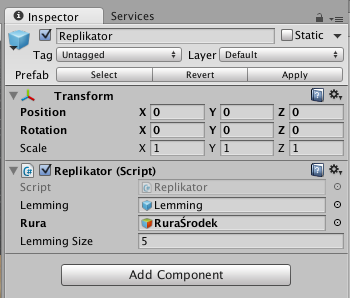
\includegraphics[width=0.7\textwidth]{images/replikator.png}
\captionof{figure}{
Konfiguracja replikatora
}
\end{center}

\begin{lstlisting}[language=CSharp]
...
public void Run () {
  StartCoroutine(Runner());
  NetworkManager.StartListening("button_left", Left);
  NetworkManager.StartListening("button_right", Right);
  NetworkManager.StartListening("button_kilof", Kilof);
  NetworkManager.StartListening("button_lopata", Lopata);
  NetworkManager.StartListening("button_jump", Jump);
  NetworkManager.StartListening("button_spadochron", Drabina);
  NetworkManager.StartListening("button_rotate", Rotate);
  NetworkManager.StartListening("button_startstop", Startstop);
  NetworkManager.StartListening("button_reset", Reset);
}

IEnumerator Runner() {
  while (lemmingCount < LemmingSize) {
    Create ();
    lemmingCount += 1;
    yield return new WaitForSeconds (secoundLimit);
  }
}
...
\end{lstlisting}
\captionof{lstlisting}{
  Uruchomienie replikatora
}

\begin{lstlisting}[language=CSharp]
...
void Left () {
  Lemming2.GetPrev ();
}

void Right () {
  Lemming2.GetNext ();
}

void Kilof () {
  if (Lemming2.activeEl) {
    Lemming2.activeEl.ToggleKilof ();
  }
}
...
\end{lstlisting}
\captionof{lstlisting}{
  Implementacja akcji
}

\subsection{Serwer komunikacyjny}
\paragraph{}
Jako technologię do obsługi połączeń zastosowano NodeJS. Obecnie jedyną zależnością zewnętrzną jest biblioteka Socket.IO \cite{socket}.
Jako manager zależności wybrano NPM. Jest on domyślnie dołączony do oprogramowania NodeJS. Aby pobrać zależności należy uruchomić polecenie ,,npm install'' w katalogu projektu.

\begin{lstlisting}[language=CSharp]
{
  "name": "server",
  "version": "1.0.0",
  "description": "",
  "main": "index.js",
  "author": "Kamil Warpechowski",
  "license": "GNU",
  "devDependencies": {
    "socket.io": "^1.4.6"
  }
}
\end{lstlisting}
\captionof{lstlisting}{
  Definicja zależności w projekcie
}

\paragraph{}
Głównym założeniem części serwerowej jest propagowanie wiadomości na linii kontroler - gra. Jednakże dzięki zastosowaniu Socket.IO możliwa jest obsługa wielu urządzeń jednocześnie. (np. dwóch kontrolerów). Dlatego też zastosowano mechanizm pokoi. Jest to grupowanie unikalnych identyfikatorów połączeń, co pozwala wysyłać komunikaty jednocześnie do wszystkich kontrolerów lub gier. Na potrzeby projektu wprowadzono limity (jedna gra, dwa kontrolery), jednakże w przyszłości jest możliwość dalszej rozbudowy.

\begin{lstlisting}[language=CSharp]
socket.on('register_controller', function () {
 if(io.sockets.adapter.rooms[CONTROLLER].length < 1) {
  console.log("register controller");
  socket.join(CONTROLLER);
 }
});

socket.on('register_game', function () {
   if(io.sockets.adapter.rooms[GAME]) {
  console.log("register game");
  socket.join(GAME);
   }
});
}
\end{lstlisting}
\captionof{lstlisting}{
  Grupowanie połączeń
}
\newpage
\begin{lstlisting}[language=CSharp]
socket.on('enable_button', function (data) {
  console.log("enable_button", data);
  io.to(CONTROLLER).emit("enable_button", data);
});
\end{lstlisting}
\captionof{lstlisting}{
  Przykład propagacji komunikatu
}
\paragraph{}
W przyszłości możliwe jest przechowywanie stanu gry na poziomie serwera (każdy kontroler może przesłać unikalny identyfikator urządzenia).

\newpage
\section{Aplikacja mobilna - kontroler}

\begin{center}
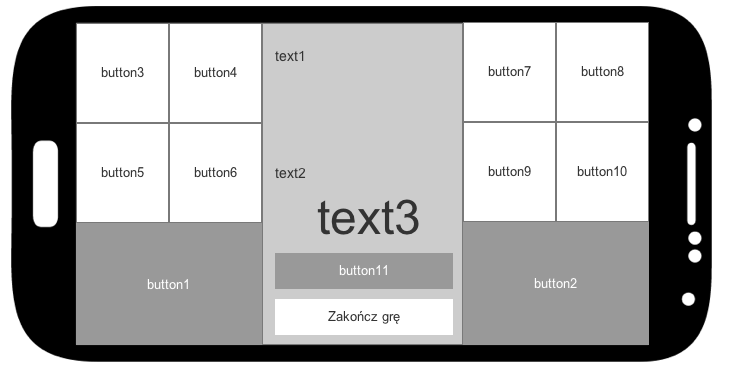
\includegraphics[width=1\textwidth]{images/button_mockup.png}
\captionof{figure}{
Makieta - układ przycisków
}
\end{center}
\paragraph{}
Głównym założeniem było stworzenie uniwersalnego kontrolera przygotowanego pod dowolny rodzaj gry, bądź innej wizualizacji stworzonej w środowisku Unity. Podczas uruchomienia kontrolera serwer wysyła statusy przycisków oraz pól tekstowych.


\begin{center}

\includegraphics[width=1\textwidth]{images/graph1.png}

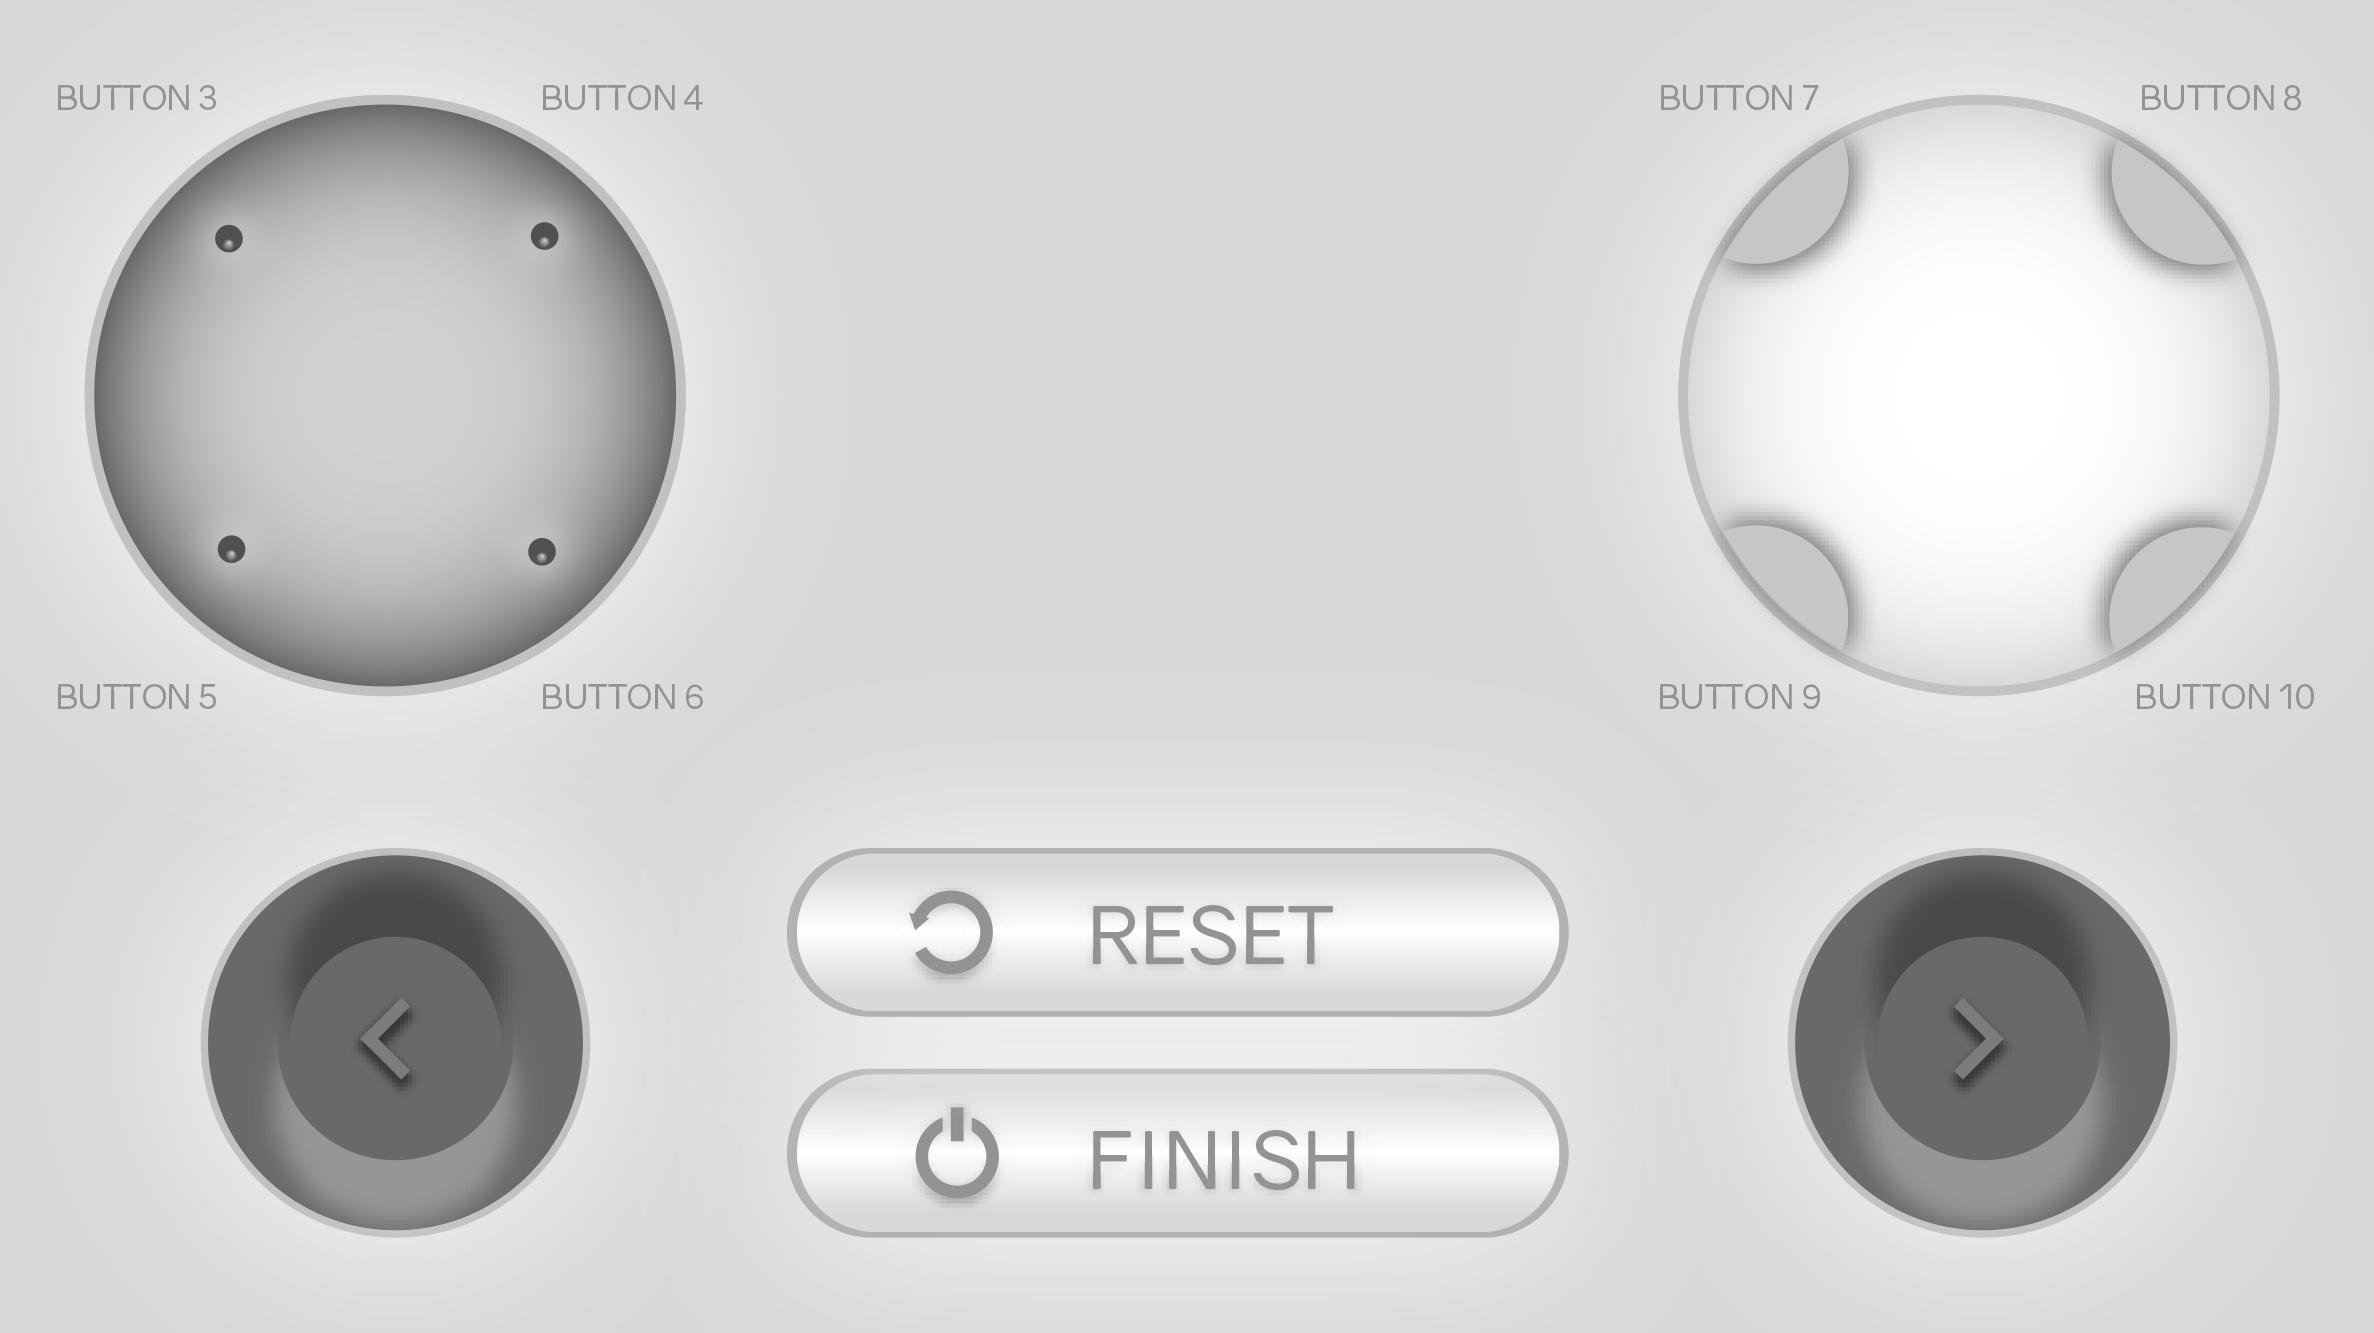
\includegraphics[width=1\textwidth]{images/graph2.png}
\captionof{figure}{
Przykładowa wizualizacja kontrolera
}
\end{center}

\subsection{Przyciski}
\paragraph{}
Każdy przycisk może zostać skonfigurowany poprzez ustawienie tekstu. Dodatkowo można zablokować przycisk podczas gdy nie jest on potrzebny w danym czasie. 
Jednym z główny założeń architektonicznych był rozdzielenie warstwy widoku od logiki biznesowej. Ustalono, że stworzenie nowego przycisku odbywać się będzie wymagało tylko dodania definicji w warstwie widoku (plik layout w formacie XML).

\begin{lstlisting}[language=XML]
<pl.pjatk.remotecontroller.CustomButton
    app:name="button2"
    android:layout_gravity="center_horizontal"
    android:layout_height="wrap_content"
    android:layout_width="wrap_content"
/>
\end{lstlisting}
\captionof{lstlisting}{
	Przykład zdefiniowanego przycisku
}
\paragraph{}
Na potrzeby realizacji powyższego założenia stworzono klasę CustomButton, która jest rozszerzeniem (dziedziczy bezpośrednio) klasy Button znajdującej się w pakiecie  android.widget.
\paragraph{}
Każdy z przycisków musi posiadać własną nazwę kodową, gdyż serwer podczas komunikacji sieciowej identyfikuje przycisk poprzez unikalny klucz. Domyślnie w środowisku Android każdy komponent wizualny może posiadać swoje Id, jednakże jest one reprezentowane poprzez liczbę typu Integer.
Dla ułatwienia dalszego rozwoju aplikacji postanowiono stworzyć nowy atrybut. Ich definicje umieszczas ię w formacie XML w pliku attrs.xml

\begin{lstlisting}[language=XML]
<resources>
    <declare-styleable name="CustomButton">
        <attr name="name" format="string" />
    </declare-styleable>
</resources>
\end{lstlisting}
\captionof{lstlisting}{
    Definicja atrybutu o nazwie name
}

\paragraph{}
W konstruktorze poza domyślnymi wywołaniami klasy bazowej Button zapisywana jest wartość atrybutu name do zmiennej o tej nazwie oraz następuje wstępna konfiguracja przycisku.

\begin{lstlisting}[language=Java]
private static HashMap<String, CustomButton> buttons = new HashMap<String, CustomButton>();

private void setUp() {
    buttons.put(getName(), this);
    setText(getName());

    setOnClickListener(new View.OnClickListener(){
        @Override
        public void onClick(View v) {
            try {
                new Runner().execute(getName());
            } catch (Exception e) {
                Toast.makeText(getContext(), R.string.SendError, Toast.LENGTH_SHORT).show();
            }
        }
    });
}
\end{lstlisting}
\captionof{lstlisting}{
    Konfiguracja w klasie CustomButton
}
\paragraph{}
{\color{red}opisac co tu sie dzieje}


\subsection{Użycie styli}
\paragraph{}
Dodatkowym wymaganiem było umożliwienie szybkiej zmiany wyglądu przycisków w trakcie działania aplikacji. Użycie natywnych styli niestety nie jest możliwe bez ponownego renderowania widoku. Aby zaoszczędzić czas i moc obliczeniową postanowiono, iż zostatnie użyta technologia zmiany tła za pomocą metody backgroundResource. Różne wyglądy przycisku mogą być definiowane jako selektory (zewnętrzne pliki xml w katalogu drawable). Ważne, by plik był odpowiednio nazwany, gdyż po nazwie następuje wyszukiwanie schematu podczas zmiany wyglądu.

\begin{lstlisting}[language=Xml]
<?xml version="1.0" encoding="utf-8"?>
<selector xmlns:android="http://schemas.android.com/apk/res/android">
    <item android:state_pressed="true" >
        <shape>
            <gradient
                android:startColor="#bf1d00"
                android:endColor="#801300"
                android:angle="270" />
            <corners android:radius="10dp" />
            <stroke
                android:width="1dp"
                android:color="#71c2eb" />
        </shape>
    </item>
    <item>
        <shape xmlns:android="http://schemas.android.com/apk/res/android"
            android:shape="rectangle">
            <gradient android:startColor="#FFFFFF"
                android:endColor="#999"
                android:angle="270" />
        </shape>
    </item>
</selector>
\end{lstlisting}
\captionof{lstlisting}{
    Przykład zdefiniowanego tła
}
\paragraph{}
Wymaganiem była jednoczesna zmiana wyglądu wszystkich przycisków. Rozwiązano to za pomocą metody statycznej, która iteruje po wszystkich przyciskach i wywołuje metdę backgroundResource.


\begin{lstlisting}[language=Java]
 public static void setLayout(int i) {
    for (CustomButton btn : buttons.values()) {
        btn.setBackgroundResource(i);
    }
}
\end{lstlisting}
\captionof{lstlisting}{
   Zmiana tła dla wszystkich przcisków
}


\begin{lstlisting}[language=Java]
CustomButton.setLayout(R.drawable.dark);
\end{lstlisting}
\captionof{lstlisting}{
   Przykład wywołania zmiany tła przycisków.
}



\subsection{Informacje tekstowe}
\paragraph{}
Pola tekstowe mogą mieć ustawioną dowolną treść w dowolnym czasie.

\subsection{Komunikacja sieciowa}
\paragraph{}
{\color{red}tutaj opisać implementacje warstwy komunikacyjnej}

\section{Środowisko uruchomieniowe}
\paragraph{}
Powyżej opisana aplikacja została uruchomiona testowo w laboratorium na Polsko-Japońskiej Akademii Technik Komputerowych.

\subsection{Aplikacja główna - Unity}
\paragraph{}
Aplikacja została uruchomiona na komputerze przenośnym (laptop) posiadającym kartę graficzną umożliwiajacą podłączenie dwóch zewnętrznych ekranów - projektorów. Pierwszy z nich został połączony za pomocą złącza cyfrowego HDMI, natomiast drugi łączem DVI.
\subsection{Serwer komunikatów}
Serwer został uruchomiony na tym samym urządzeniu co aplikacja główna. Do uruchomienia nezbędne było zainstalowanie Node.JS wraz z menadżerem zależności - NPM.
\subsection{Aplikacja mobilna - kontroler}
\paragraph{}
Kontroler został uruchomiony na urządzeniu Xiaomi Mi4c wyposażonym w system Android w wersji 5.1. Urządzenie sprawdziło się jako kontroler, gdyż posiada ekran o rozmiarze 5 cali. Ilość pamięci operacyjnej była wystarczająca. Aplikacja zużywała tylko około 2-4\% pamięci RAM. 
\newpage
\section{Inne implementacje - Google Cardboard}
\paragraph{}
Innym przykładem implementacji projektu w rozszerzonej rzeczywistości może być platforma Google Cardboard \cite{cardboard}. Są to niskobudżetowe okulary stworzone przez firmę Google do wyświetlania wirtualnej rzeczywistości. Kartonowe okulary powstały w celu wyświetlania obrazu stereoskopowego. Posiadają one miejsce do umieszczenia dowolnego telefonu komórkowego typu smartphone. Do projektu wybrano wersję, która pozwala na umieszczenie telefonu w sposób taki, iż tylna kamera nie jest zasłonięta przez obudowę. Dzięki temu można użyć platformę Cardboard przeznaczoną pierwotnie tylko do wirtualnej rzeczywistości do stworzenia aplikacji wykorzystującą augmented reality.

\begin{center}
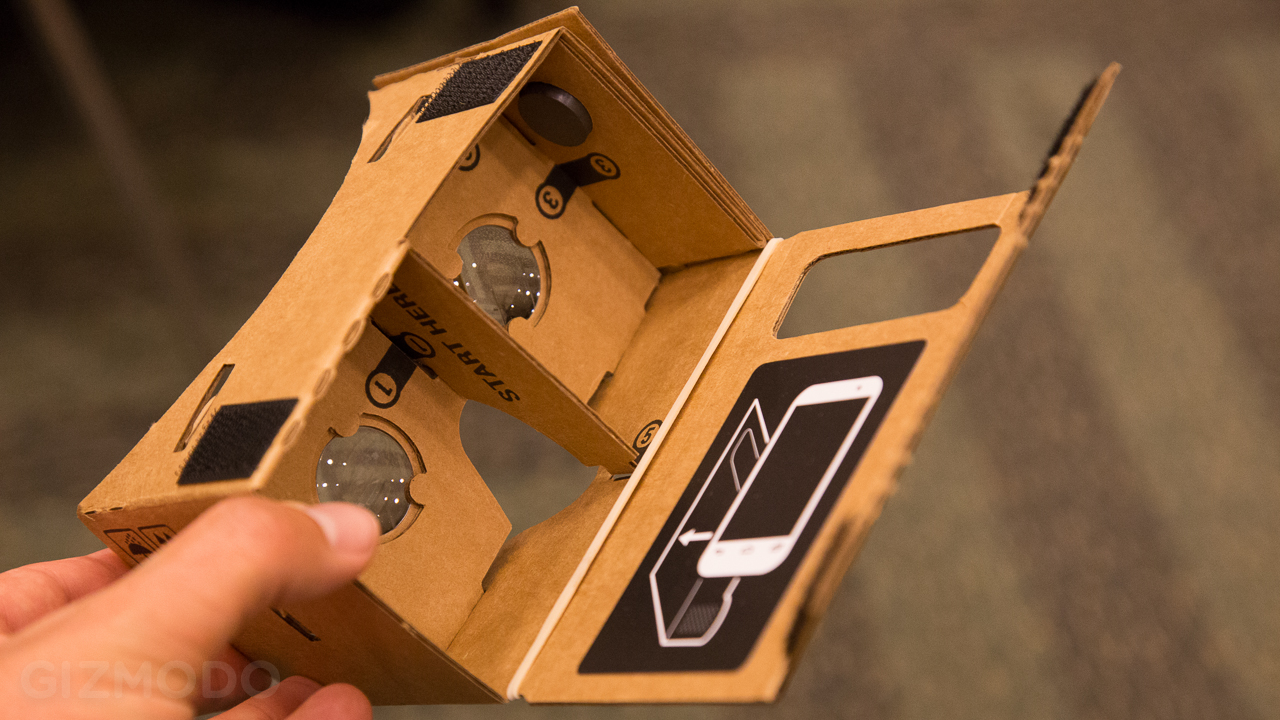
\includegraphics[width=1\textwidth]{images/cardboard.jpg}
\captionof{figure}{
Google Cardboard w wersji do samodzielnego złożenia\cite{gizm}
}
\end{center}

\paragraph{}
Dzięki użyciu kamery użytkownik widzi obraz znajdujący się przed nim. Aby obraz był stereoskopowy należało stworzyć aplikację, która wyświetlić strumień danych z kamery dzieląc go na dwa obrazy (kolejno dla lewego oraz prawego oka).

\begin{center}
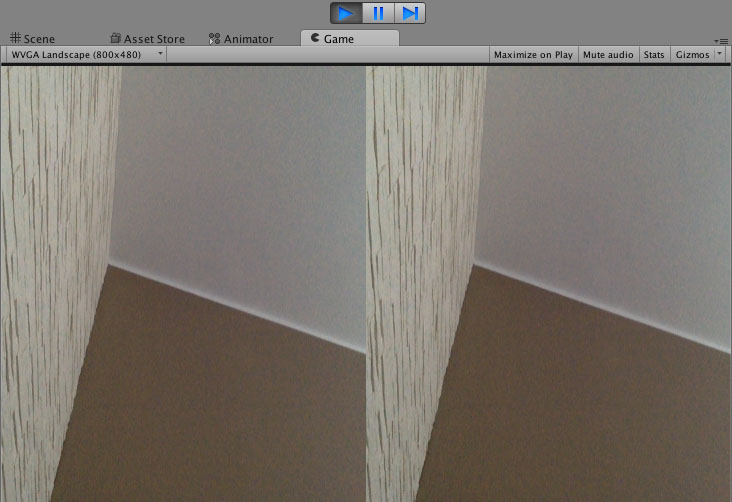
\includegraphics[width=1\textwidth]{images/kadr.jpg}
\captionof{figure}{
Ujęcie z kamery aparatu w obrazie stereoskopowym - scena w Unity
}
\end{center}

\subsection{ArToolkit}
\paragraph{}
W celu wyświetlenia wirtualnych obiektów na obrazie z kamery rozbudowano aplikację z porzednich rozdziałów. Do platformy Unity doinstalowano zewnętrzny komponent ARToolKit\cite{ar}. Jest to biblioteka wydana przez University of Washington\cite{ar2}, lecz obecnie upostępniona jest na licencji GNU. Kod źródłowy jest otwarty i rozwijany przez środowisko Open Source\cite{ar3}.
\subsection{Markery}
\paragraph{}
Za pomocą tej biblioteki możliwe jest wykrywanie w obrazie z kamery markerów, czyli specjalnie przygotowanych czarno-białych obrazków (w naiwnej implementacji - wydrukowanych na kartkach), oraz nakładanie w ich miejsce trójwymiarowych modeli lub całych scen. Dzięki bibliotece ArToolkit możliwe jest diagnozowanie pod jakim kątem padania oraz w jakiej odległości od urządzenia znajduje się marker. Umiejscowienie tagu analizowane jest w czasie rzeczywistym, co zapewni ciągłą korekcję ułożenia wirtualnych modeli względem ich realnych odpowiedników.

\begin{center}
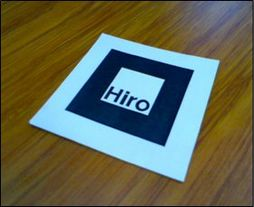
\includegraphics[width=1\textwidth]{images/hiro.png}
\captionof{figure}{
Przykład przygotowanego obrazka do rozpoznawania - marker
}

\end{center}
\paragraph{}
Szablony markerów można wykonywać we własnym zakresie. Aby zaimportować nowe obrazki do biblioteki ArToolkit należy przygotować specjalny plik binarny reprezentujący model markera\cite{marker}.

\begin{center}
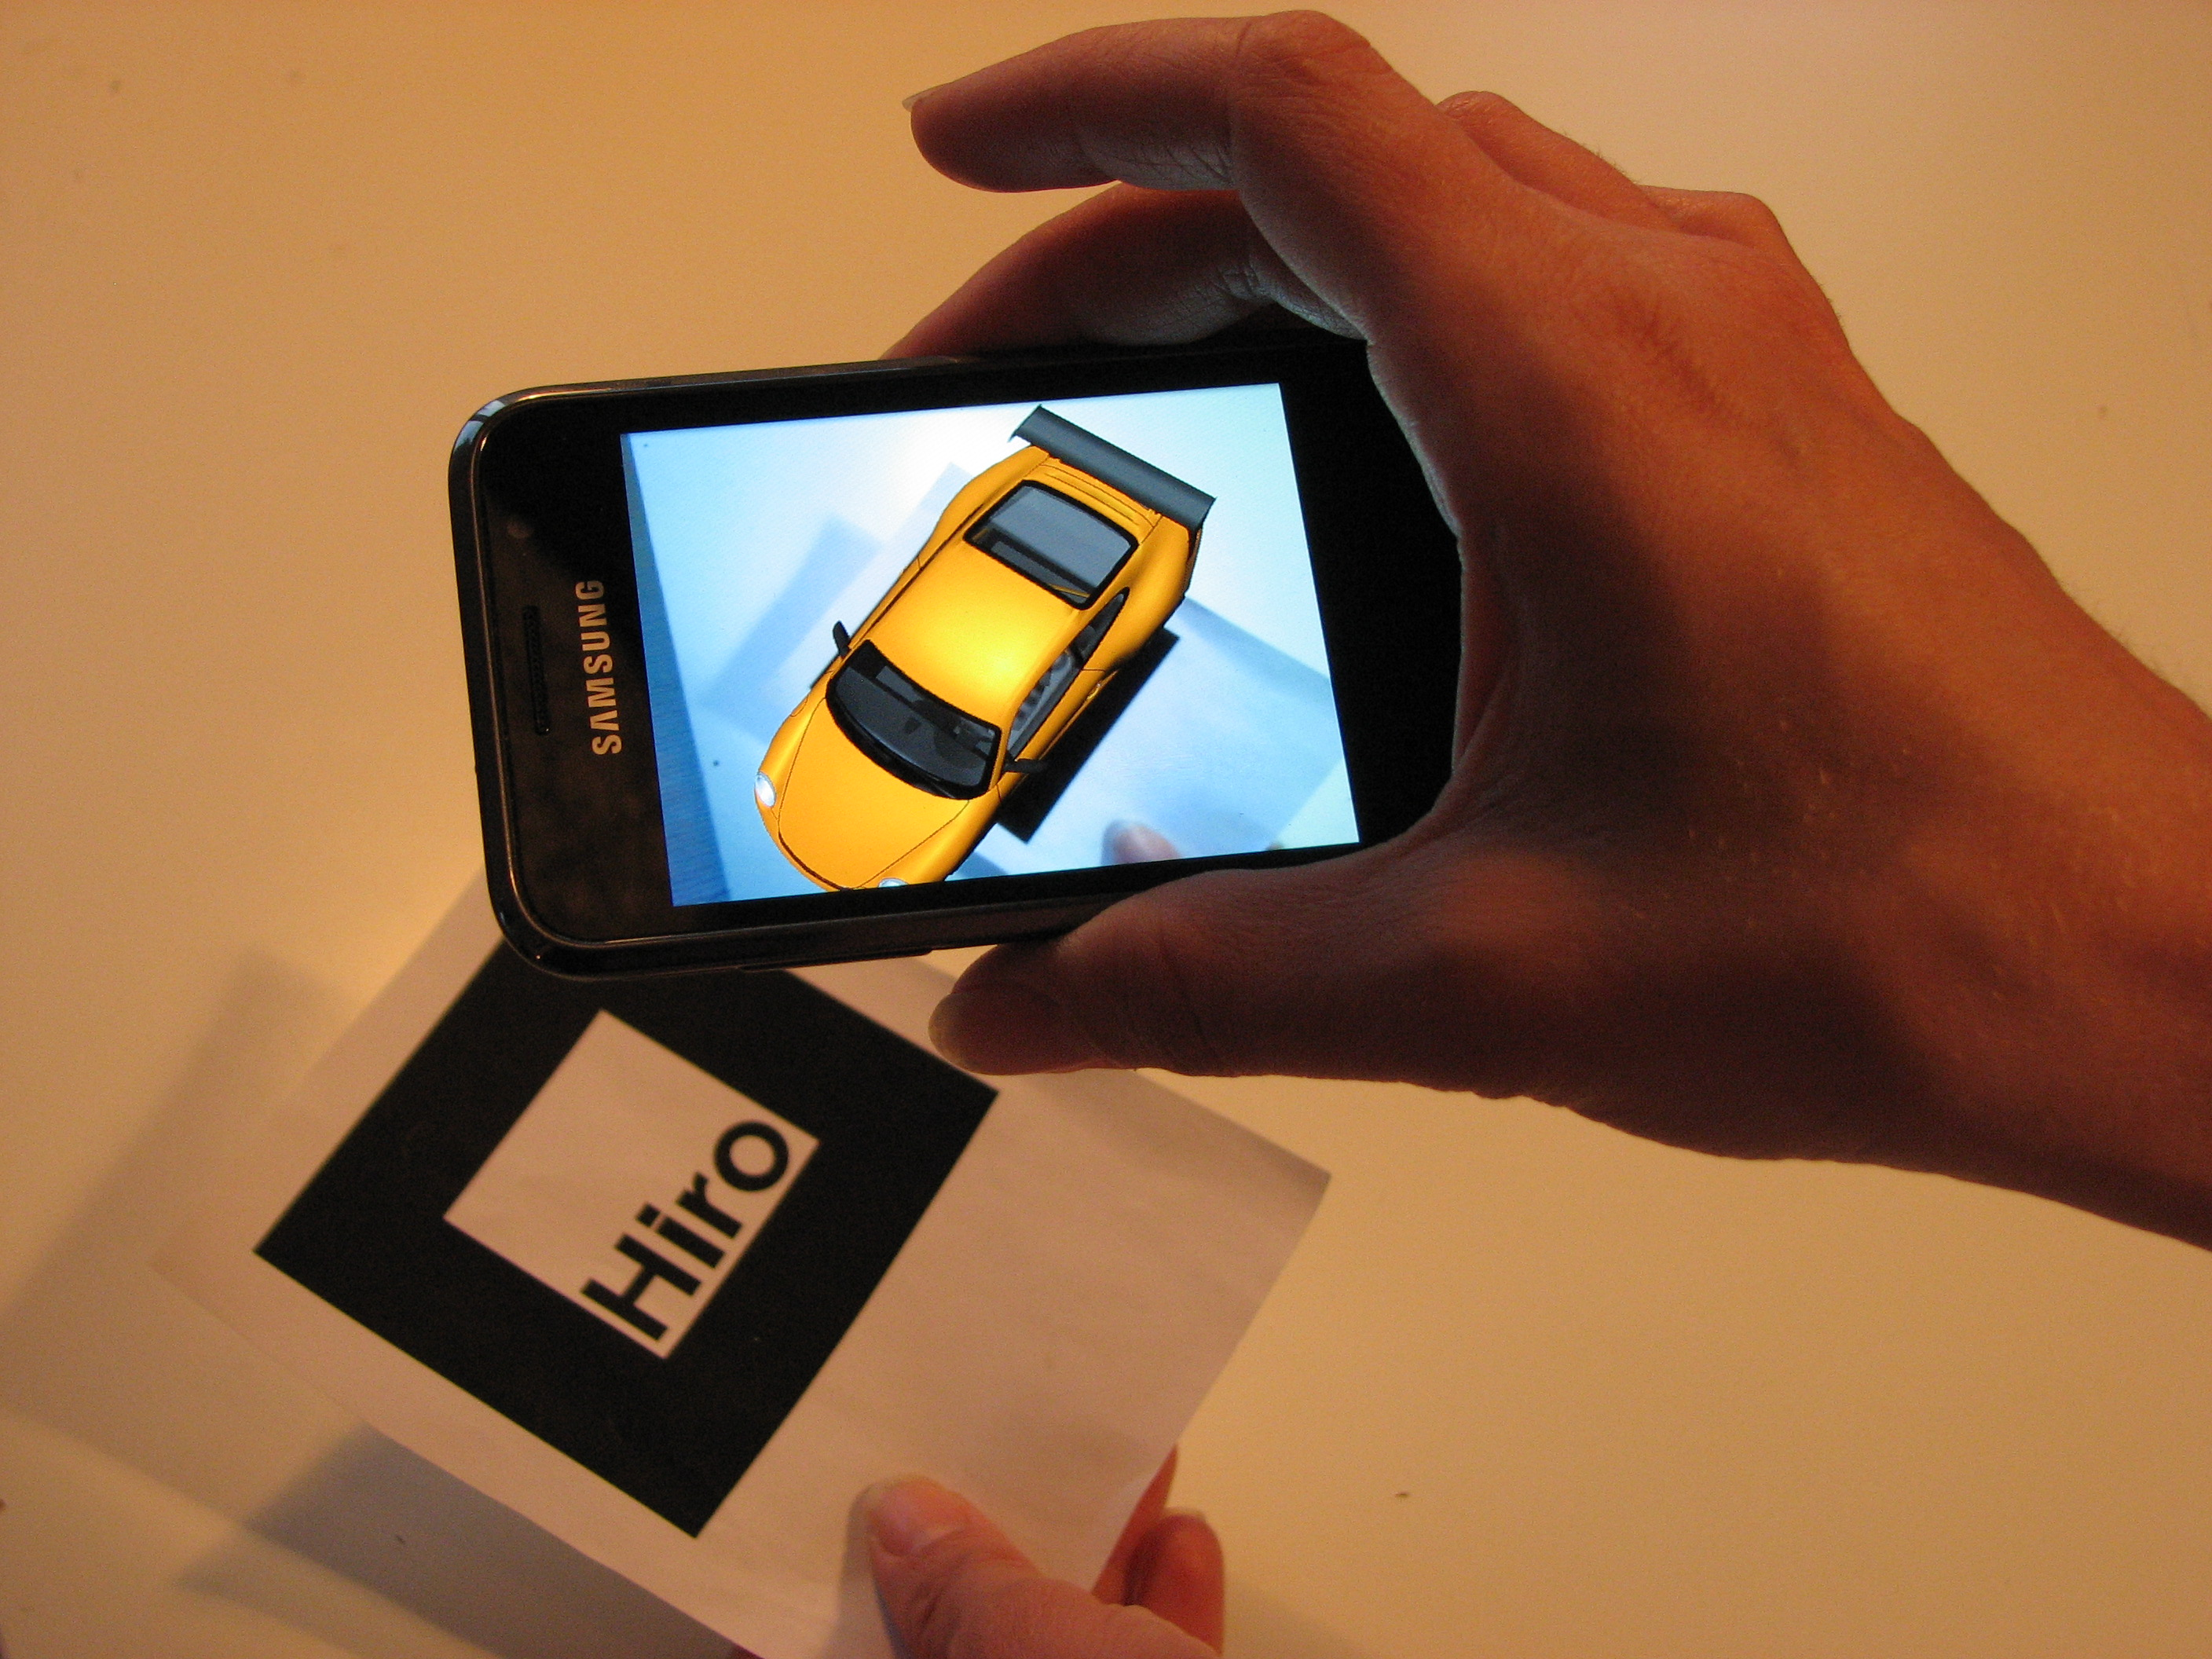
\includegraphics[width=1\textwidth]{images/artoolkit-demo.jpg}
\captionof{figure}{
Przykład zastosowania markera w ARToolkit\cite{cardboard2}
}
\end{center}
\subsection{Przykład implementacji}
\begin{center}
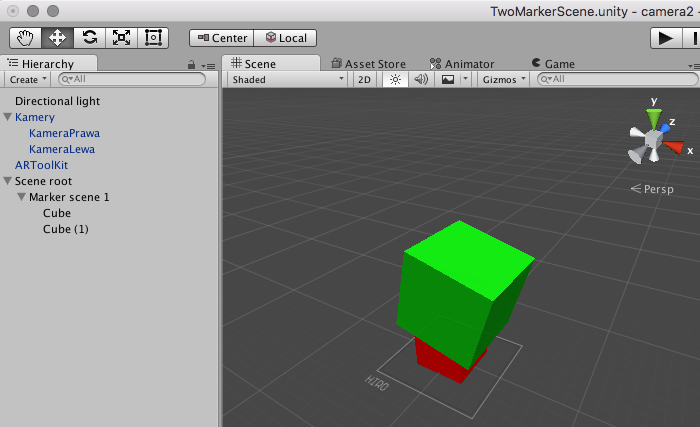
\includegraphics[width=1\textwidth]{images/artoolkit-przyklad.png}
\captionof{figure}{
Podstawowa impementacja
}
\end{center}
\paragraph{}
Implementacja na platformie Unity przy użyciu ArToolkit jest zasadniczo prosta. Przy użyciu wcześniej przygotowanych kodów markerów (domyślnie dostępne są dwa) i zastosowaniu prefabrykatów w trójwymiarowej przestrzeni można wskazać miejsce od którego będzie odliczana odległość do pozostałych elementów. np. Jeżeli bryła ustawiona zostanie w odległości 5cm od prefabrykatu to podczas analizy obrazu i wykryciu rzeczywistego markera to bryła zostanie umiejscowiona na ekranie w tej samej odległości.
\subsection{Napotkane problemy i ograniczenia}
\paragraph{}
\begin{enumerate}
	\item Proces renderowania musi odbywać się na telefonie komórkowym, gdyż obraz kamery jest ciągle analizowany. Przy dużych scenach stworzonych w Unity moc obliczeniowa urządzenia jest niewystarczająca.
	\item Analizowanie pozycji markera przy nieustannie włączonej kamerze powoduje dużą drenację baterii urządzenia. Czas pracy na baterii jest mocno ograniczony
	\item Unity w wersji Personal (darmowej) skompilowanej pod platrformę mobilną (np. Android) nie udostępnia obsługi sieci (np. za pomocą połączenia TCP). Nie pozwala to na połączenie z zenętrznym kontrolerem.
	\item Sterowanie za pomocą kontrolera bez fizycznych przycisków z założonymi okularami Google Cardboard jest bardzo uciążliwe. W przyszłości należałoby rozważyć połączenie telefou z zewnętrznym kontrolerem typu PAD\cite{pad}.
\end{enumerate}
\newpage
\section{Inne implementacje - Project Tango}
\paragraph{}
Kolejnym przykładem implementacji może być platforma Google Project Tango\footnote{https://get.google.com/tango/}. Jest to platforma rozszerzonej rzeczywistości zapoczątkowana przez Johny'ego Lee (współtwórcy między innymi Microsoft Kinect\footnote{https://en.wikipedia.org/wiki/Johnny\_Lee\_(computer\_scientist)}) w 2014. 
\paragraph{}
Idea projektu jest bardzo podobna jak przykład zaprezentowany w poprzednim rozdziale. Jednakże Project Tango to również podzespoły sprzętowe. Twórcy zastosowali specjalne kamery do pomiaru głębi oraz analizy ruchu (technologia podczerwieni). Kamery te korzystają z technologii Intel Real Sense. Dzięki temu urządzenie potrafi analizować obraz kamery i mapować go na trójwymiarowy obraz. Z dokładnością do milimetra urządzenie jest w stanie określić wymiary realnych elementów znajdujących się przed kamerą. Dzięki temu nie ma potrzeb używania zbędnych fizycznych markerów do określenia miejsca w którym znajduje się odbiorca z urządzeniem.
\paragraph{}
Firma Google zaprezentowała projekt w 2014 roku wraz z dwoma urządzeniami testowymi (The Yellowstone tablet,  The Peanut phone). Jednakze te urządzenia nie trafiły nigdy na rynek kompercyjny. Dopiero w 2016 roku firma Lenovo zaprezentowała pierwszy masowo produkowany telefon obsługujący Project Tango - Lenovo Phab2 Pro.
\paragraph{}
Projekt pod początku udostępnia developerom możliwość tworzenie aplikacji za pomocą API do języków Java oraz C. Dodatkowo udostępniona jest SDK (Software Development Kit) wraz z obszerną dokumentacją do platformy Unity \footnote{https://developers.google.com/tango/apis/unity/}.
\paragraph{}
Jedynym środowiskiem uruchomieniowym dostępnym na obecną chwilę jest Android, chociaż Google zapowiada możliwość w przyszłości uruchomienia w środowisku Windows 10.

\begin{center}
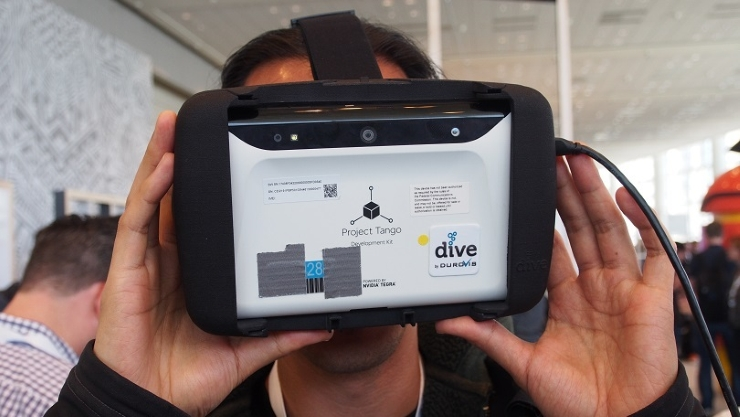
\includegraphics[width=0.9\textwidth]{images/tango.jpg}
\captionof{figure}{
Prototyp urządzenia
}
\end{center}

\paragraph{}
Google zaprezentowało również okulary do wirtualnej rzeczywistości. Jednakże był to tylko prototyp. Obecnie na rynku nie ma urzędzenia dostosowanego do tego celu. Jedyną możliwością byłoby użycie Lenovo Phab Pro wraz z Google Cardboard.

\subsection{Wady i zalety}
\paragraph{}
\begin{enumerate}
	\item Project Tango jest stworzony jako kooperacja dedykowanego sprzętu oraz specjalistycznego oprogramowania, co za tym idzie wydajność urządzeń powinna być duża.
	\item Dużą wadą jest to, iż na rynku dopiero pojawił się pierwszy smartphone z obsługą projektu. Technologia wydaje się być na początkowej fazie rozwoju.
	\item Dzięki tej technologii można zrezygnować z markerów opisanych w poprzednim rozdziale. Odczucia użytkowników powinny być bardziej intuicyjne.
\end{enumerate}
\newpage
\section{Wnioski i dalszy rozwój}
\paragraph{}
Obserwując rynek nowych technologii można zauważyć duże zainteresowanie zarówno rozszerzoną jak i wirtualną rzeczywistością. Producenci eksperymentują z różnymi urządzeniami, jednakże większość ich jest w fazie testów i nie jest dostępna dla potencjalnych konsumentów.
Wiele z firm próbuje tworzyć własne standardy, jednakże żaden 


\paragraph{}
{\color{red}Napisać o tym, ze Microsoft otworzyl platforme hololens, wiec w przyszłosci będą nowe urządzenia}


\newpage
\thispagestyle{empty}
  
\listoffigures
\listoftables
\lstlistoflistings


\begin{thebibliography}{99}
\bibitem{pa} Building Microservices,  Sam Newman , Wydanie 4, 2016
\end{thebibliography}

\end{document}
